\documentclass[a4paper, ]{article}
\usepackage[left=2cm, right=2cm, bottom=2.5cm, top=2.5cm]{geometry}

\usepackage[utf8]{inputenc}
\usepackage{amsmath}
\usepackage{amsfonts}
\usepackage{wasysym}
\usepackage{amssymb}
\usepackage{commath}
\usepackage{lipsum}
\usepackage{adjustbox}
\usepackage{float}
\usepackage{hyperref}
\usepackage{graphicx}
\usepackage{gensymb}
\usepackage[spanish]{babel}

\usepackage{multicol}
\usepackage{listings}
\usepackage{enumitem}
\usepackage{booktabs}

\usepackage{multicol}
\title{\Huge{\vspace{-1em}La(s) hoja(s) de Chema}}
\author{}
\date{}
\makeatletter



\usepackage[dvipsnames]{xcolor}

\usepackage{wrapfig}
\usepackage{cancel}

\usepackage{fancyhdr}
\pagestyle{fancy}
\lhead{Alex Martínez Ascensión}
\chead{}
\rhead{\today}


\usepackage{fourier}

\usepackage[T1]{fontenc}
%\usepackage[default]{gillius}
\usepackage{Alegreya}


\setlength{\parskip}{1em}
\setlength{\parindent}{0em}

\usepackage[
type={CC},
modifier={by-nc-nd},
version={3.0},
]{doclicense}

\setlength{\parindent}{0em}
\setlength{\parskip}{1.1em}
\renewcommand{\baselinestretch}{1.15}
\setlength\itemsep{0em}


\newenvironment{itemizex}%
{\begin{itemize}[noitemsep]%
		\setlength{\itemsep}{0 em}%
		\setlength{\parskip}{0pt}
				\vspace*{-1em}
	}%
	{\end{itemize}\vspace*{-1em}}



\newcommand{\dd}{\ensuremath{\operatorname{d}}}
\renewcommand{\d}[1]{\ensuremath{\operatorname{d}\!{#1}}}
\newcommand{\R}{\mathbb{R}}
\renewcommand{\P}{\mathbb{P}}
\renewcommand{\H}{\mathbb{H}}
\newcommand{\E}{\mathbb{E}}
\newcommand{\m}{\text{medio}}
\newcommand{\iso}{\text{Isom}}
\newcommand{\sen}{\text{sen}}
\usepackage{calrsfs}
\DeclareMathAlphabet{\pazocal}{OMS}{zplm}{m}{n}
\newcommand{\C}{\pazocal{C}}
\newcommand{\PP}{\pazocal{P}}
\renewcommand{\L}{\pazocal{L}}

\definecolor{azul}{HTML}{107896}
\definecolor{naranja}{HTML}{C2571A}
\definecolor{rojo}{HTML}{9A2617}
\definecolor{amarillo}{HTML}{BCA136}
\definecolor{verde}{HTML}{829356}
\definecolor{gris}{HTML}{909090}
\definecolor{rosa}{HTML}{F9A7B0}
\definecolor{amarillochillon}{HTML}{FBB117}

\newcommand{\axioma}[1]{\textcolor{naranja}{\textbf{Axioma #1}}}
\newcommand{\tma}[1]{\textcolor{rojo}{\textbf{Teorema #1}}}
\newcommand{\defi}[1]{\textcolor{azul}{\textbf{Definición #1}}}
\newcommand{\obs}[1]{\textcolor{verde}{\textbf{Observación #1}}}
\newcommand{\ejem}[1]{\textcolor{verde}{\textbf{Ejemplo #1}}}
\newcommand{\ej}[1]{\textcolor{amarillo}{\textbf{Ejercicio #1}}}
\newcommand{\lema}[1]{\textcolor{rosa}{\textbf{Lema #1}}}
\newcommand{\cor}[1]{\textcolor{rosa}{\textbf{Corolario #1}}}

\newcommand{\dem}[1]{\textcolor{gris}{\normalsize{Demostración. #1}}}

\newcommand{\importante}{\textcolor{amarillochillon}{\textbf{\danger} \,}}
\newcommand{\obligatorio}{\textcolor{rojo}{$\blacksmiley$} \,}
\newcommand{\prodvec}[1]{\langle #1 \rangle}

\begin{document}
		\maketitle

	\fontsize{12pt}{12pt}\selectfont
	\vspace*{-4em}
	
	\begin{multicols}{2}
	[
	\section{Espacios métricos}
	]
	
	\defi{1.1} $\delta: M \times M \rightarrow \R $ es una métrica o \textbf{distancia} si cumple que 
	\begin{itemizex}
		\item $\delta(x,y) > 0$ si $x \neq y$, o $\delta(x,x) = 0$
		\item $\delta(x,y) = \delta(y,x)$
		\item $\delta(x,z) \le \delta(x,y) + \delta(y,z)$
	\end{itemizex}
	
	\ej{1.1} Por inducción, la desigualdad triangular se puede generalizar a: $\delta(p^1, p^n) \le \delta(p^1, p^2) + \cdots + \delta(p^{n-1}, p^n)$
	
	\tma{1.4} Si $M' \subset M$ y existe el espacio métrico $(M, \delta)$, entonces también existe $(M', \delta)$, y se llama \textbf{métrica inducida} por $(M,\delta)$.
	
	\defi{1.5} Sean $(M,\delta), (M', \delta')$ y $g: M \rightarrow M'$. Se dice que $g$ conserva las distancias si $\delta'(g(x), g(y)) = \delta(x, y)\;\; \forall \; \; x,y \in M$. Si además $g$ es biyectiva, entonces es una \textbf{isometría}.
	
	\tma{1.7} Si existen $(M, \delta), (M', \delta'), (M'', \delta'')$ y $g: M\rightarrow M'$ y $h: M\rightarrow M'$ son isometrías, entonces $h\circ g$ y $g^{-1}$ también son isometrías.
	
	\defi{1.8} La composición de isometrías forma un \textbf{grupo} pues
	\begin{itemizex}
		\item $(g \circ h) \circ i = g \circ (h \circ i)$
		\item Si $g \in \text{Isom}(M)$ entonces $g^{-1} \in \text{Isom}(M)$
		\item La isometría identidad, $\text{id}_M \in \text{Isom}(M)$
	\end{itemizex}
	
	\defi{1.12} Si $(M, \delta)$, para $a,b \in M$ se llama \textbf{segmento} de extremos $a$ y $b$ y se representa por $[a,b]$ al conjunto $[a,b] = \{x \in M \;|\; \delta(a,x) + \delta(x,b) = \delta(a,b) \}$. Asimismo, $x,y,z \in M$ están alineados si ($x < y < z$) $y \in [x,z]$.	 
	
	\ej{1.5} Para $\sigma \in \{1,-1\}$ y $\tau \in \R$, la aplicación $f(x) = \sigma x+\tau$ es una isometría para $(\R, d_{\R})$
	

	 
	 
	 
	 
	 
	 
	 
	\end{multicols}
	
	\pagebreak
	\textcolor{gris}{\textit{Page intentionally left in blank}}
	\newpage
	\pagebreak
	
	
	\begin{multicols*}{2}
	[\section{Axiomas para la geometría euclidiana plana}]
		\axioma{P1} Si tenemos el conjunto $\P$, denominado \textbf{plano}, y la aplicación $d:\P \times \P \rightarrow \R$ llamada \textbf{distancia}, entonces$(\P, d)$ es un espacio métrico.

\defi{2.2} Una \textbf{recta} $r \subset \P$ satisface
\begin{itemizex}
	\item $r$ contiene al menos dos puntos.
	\item Para toda terna de puntos $A, B, C$, están alineados si están en $r$.
\end{itemizex}

\axioma{P2} $\P$ contiene al menos tres puntos no alineados; y por dos puntos distintos, $A$ y $B$ de $\P$ pasa una recta, $r_{AB}$.

\defi{2.6} / \tma{2.7} Dos rectas se cortan si sólo tienen un punto en común, y si no tienen ningún punto en común, entonces se denominan \textbf{paralelas}, y se denota por $a \parallel b$. Dos rectas, o se cortan o son paralelas.

\importante\axioma{P3} Para toda recta $r \subset \P$ existe una biyección $\gamma: r \rightarrow \R$ tal que $|\gamma(X) - \gamma(Y)| = |x - y| = d(X, Y) \;\; \forall \;\; X,Y \in r$ 

\obs{2.8} Si $A, B \in r$ son distintos, entonces existe un punto $M\in r: d(A,M) = d(M,B)$ que denotamos por $\m[A,B]$ y se llama \textbf{punto medio}. Asimismo sólo existe un punto $B \in r$ tal que $B = \m[A, M]$.

\obs{2.9} Si $r$ es una recta y $P \in r$, entonces $r$ se puede dividir en dos \textbf{semirrectas}, que son los conjuntos $\{X \in r \; | \; \gamma(X) > \gamma(P)\}$ y $\{X \in r \; | \; \gamma(X) < \gamma(P)\}$.

\axioma{P4} Para toda recta $r \subset \P$ hay dos subconjuntos $H^1$ y $H^2$, denominados \textbf{semiplanos} de $r$, que verifican:
\begin{itemizex}
	\item $H^1 \cup H^2 = \P-r$
	\item Si $X,Y \in H^i$ entonces $[X,Y] \subset H^i$
	\item Si $X \in H^1$ y $Y \in H^2$ entonces $[X,Y] \cap r \neq \emptyset$.
\end{itemizex}

\defi{2.15} Sean $P, Q, R$ no alineados, entonces el triángulo $\triangle\{P,Q,R\}$, o $\triangle PQR$ está formado por los segmentos $[P,Q]$, $[Q,R]$, $[P,R]$, llamados lados, y los vértices $P,Q, R$.

\tma{2.16 [Axioma de Pasch]a} Dado un triángulo $\triangle PQR$ y una recta $r$; si $r$ corta a $[P,Q]$, entonces o corta a $[P,R]$ o a $[Q, R]$.

\defi{2.17 = 1.5} Una \textbf{isometría} en $\P$ es una biyección $g: \P \rightarrow \P$ que cumple que $d(g(X), g(Y)) = d(X,Y) \;\;\forall\;\; X,Y \in \P$.

\tma{2.18} Si $A,B \in \P$ y $g \in \iso(\P)$ entonces $g([A,B]) = [g(A), g(B)]$ y $g(r_{AB}) = r_{g(A)g(B)}$ 

\axioma{P5} Si $A_1, A_2 \in \P$ y $B_1, B_2 \in \P$ son dos pares de puntos que cumplen $d(A_1,A_2) = d(B_1,B_2)$ entonces existe $g \in \iso(\P)$ tal que $g(A_i) = B_i$. Se dice que esos pares de puntos son \textbf{congruentes}.

\axioma{P6} Para toda recta $r$ existe una isometría $\sigma$ llamada \textbf{reflexión} tal que  
\begin{itemizex}
	\item $\sigma(X) = X\iff X \in r$
	\item $\sigma \circ \sigma = \text{Id}$
\end{itemizex}


\defi{2.23} / \tma{2.25} / \cor{2.30} Una recta $l$ es \textbf{ortogonal} a $r$ si para todo $S \in l$ y para todo par de puntos $A, B$ que cumple que $M = \m[A,B]$, de modo que $l \cap r = M$, entonces se da que $d(A,S) = d(S,B)$. Se denota $l \perp_M r$. En estas condiciones, $l = \{X \in \P \; | \; d(S,A) = d(S,B)\}$, se denomina \textbf{mediatriz} de $[A,B]$. 

\begin{figure}[H]
	\centering
	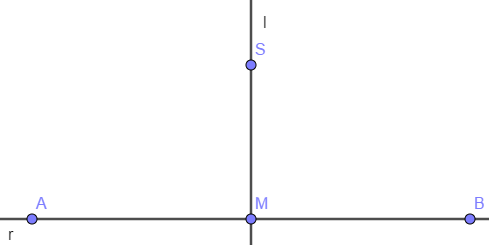
\includegraphics[width=7cm]{figuras/2-23.png}
	\vspace{-1em}
\end{figure}

\lema{2.21} Si $\sigma_r$ entonces, para todo $X$, $\m[X, \sigma_r(X)] \in r$.

\obs{2.24} Si $l \perp r$ y $g \in \iso(\P)$ entonces $g(l) \perp g(r)$.

\importante\tma{2.26} Si $l, r \subset \P$ cortan en $M$ y $\sigma_l, \sigma_r$ son dos reflexiones de $l$ y $r$, entonces se cumple que $l \perp_M r \iff r \perp_M l \iff \sigma_r(l) = l \iff \sigma_l(r) = r$.

\importante\tma{2.27 / 2.29} Para toda recta $r$ y todo punto $S \in \P - r$, existe una recta $l$ ortogonal a $r$, que pasa por $S$. Si $r$ es una recta, y $M \in r$, entonces existe $l$ tal que $l \perp_M r$.

\axioma{P7} Para toda recta $r$ y todo punto $P$ existe sólo una recta \textbf{paralela} a $r$ que pase por $P$.

\tma{2.31 / 2.33} Si $a \perp l$ y $b \perp l$ entonces $a \parallel b$. Sean $a \parallel b$. Entonces, para todo $A \in a$, la única recta $l \perp_A a$ también es ortogonal a $b$.

\tma{2.32} Las rectas parallelas forman una relación de equivalencia.
\begin{itemizex}
	\item Reflexividad: $a\parallel a$
	\item Simetría: $a \parallel b \rightarrow b \parallel a$
	\item Transitividad  $a \parallel b $ y  $b \parallel c \rightarrow a \parallel c$
\end{itemizex}

\ej{2.6} Sean $A,B \in r$, $A \neq B$. Para todo $t$, existe un único $P_t\in r$ que cumple $d(P_t,A) = \abs{t}$ y $d(P_t, B) = \abs{t-d(A,B)}$. En definitiva, la posición de $P_t$ está sólamente determinada por las distancias $d(A, P_t)$ y $d(P_t, B)$.
	 
	 
	 
	 
	 
	 
	 \end{multicols*}\pagebreak


	\begin{multicols*}{2}
	[\section{Isometrías del plano}]
	
\defi{3.1} Para una aplicación $\phi: \pazocal{M} \rightarrow \pazocal{M}$, $P\in \pazocal{M}$ es un \textbf{punto fijo} de $\phi$ si $\phi(P) = P$; y $\pazocal{D} \subset \pazocal{M}$ es un \textbf{subconjunto invariante} de $\phi$ si $\phi(\pazocal{D}) = \pazocal{M}$.

\lema{3.2} Si $g \in \iso(\P)$ y $A \neq B$ son dos puntos fijos de $g$, entonces todo $X \in r_{AB}$ es punto fijo de $g$.


\defi{3.3} Si $g, g' \in \iso(\P)$, $g$ y $g'$ son \textbf{conjugadas}
si existe una isometría $h$ tal que $gh = hg' \iff g = hg'h^{-1}$.

\tma{3.4} Un punto $P$ es fijo de $g$ sii $h^{-1}(P)$ es un punto fijo de $g'$.

\dem{Si $h^{-1}(P)$ es punto fijo de $g'$, entonces $g'(h^{-1}(P)) = h^{-1}(P)$. Por tanto, $g(P) = hg'h^{-1}(P) = hh^{-1}(P) = P$, luego $g(P) = P$.}

\ejem{3.5} Una reflexión sobre $r$ cumple que
\begin{itemizex}
	\item $\sigma_r\circ\sigma_r = \text{id}_{\P}$ y $\sigma_r(X) = X \iff X \in r$ (\axioma{P6})
	\item $\sigma_r(H^1) = H^2$ y viceversa.
	\item $X$ y $\sigma_r(X)$ se encuentran en una recta ortogonal a $r$.
\end{itemizex} 

\tma{3.6} Sea $g\in \iso(\P)$ y sea $r_{AB}$. Si $A, B$ son puntos fijos en $g$, entonces o bien $g = \sigma_r$ o bien $g = \text{id}_\P$. 

\tma{3.9} Llamamos $\rho$ una \textbf{rotación} a una isometría que tiene un punto fijo $C$. Para toda recta $a$ pasando por $C$ existen dos rectas $b, b'$ únicas tales que $\rho = \sigma_b\sigma_a = \sigma_a\sigma_{b'}$.

\begin{figure}[H]
	\centering
	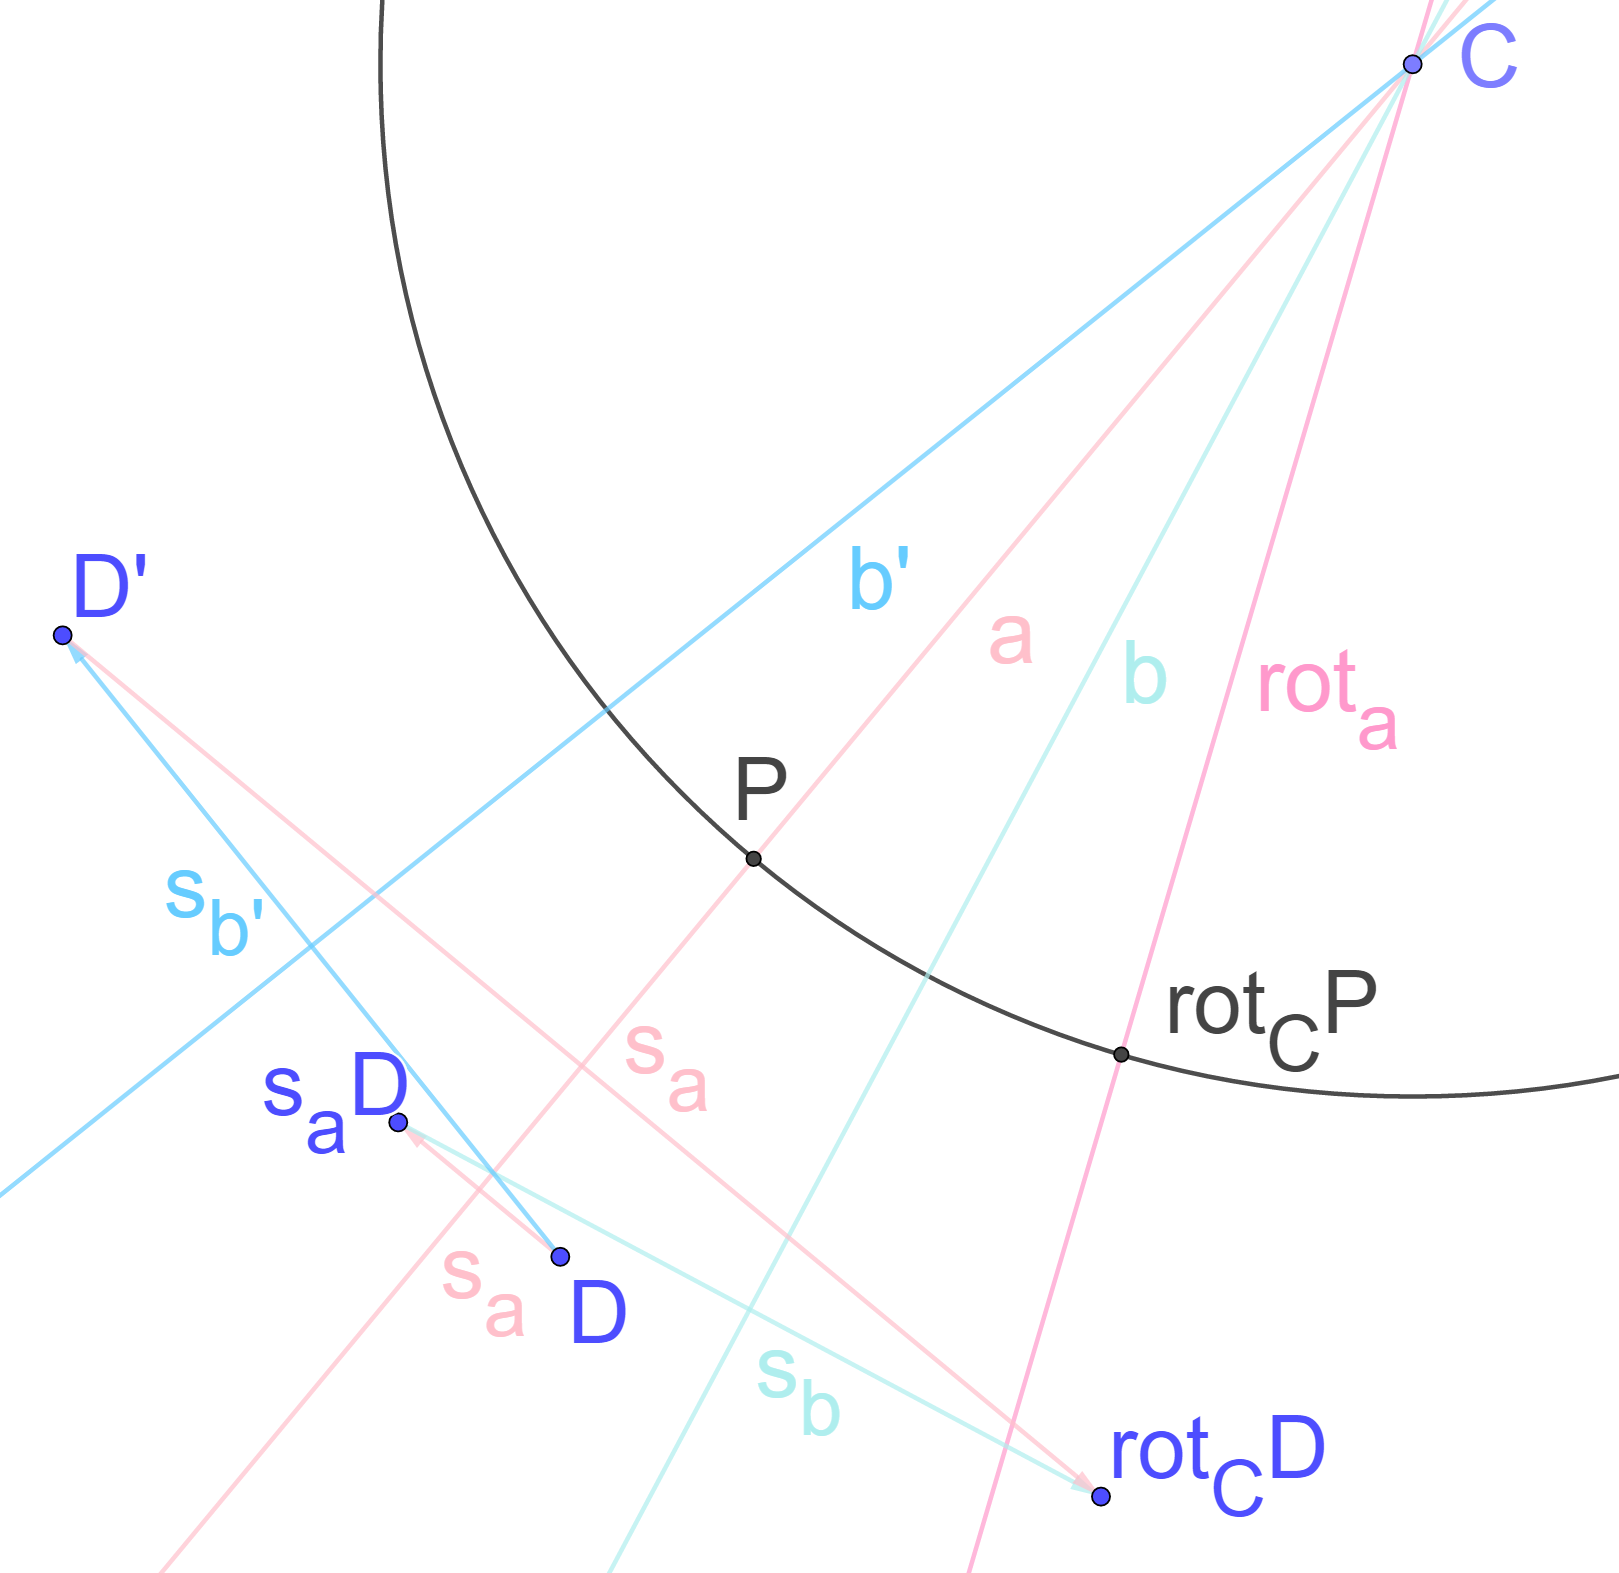
\includegraphics[width=7cm]{figuras/3-9.png}
	\vspace{-1em}
\end{figure}

\ej{3.1} Llamamos $\tau$ una \textbf{traslación} a una isometría que no tiene puntos fijos y deja una recta $c$ invariante, es decir, $\tau(c) = c$. entonces para toda recta $a\perp c$ existen dos rectas $b,b' \perp c$ que cumplen $\tau = \sigma_b\sigma_a = \sigma_a\sigma_{b'}$. Además, si $\tau(l) = l$, entonces $l \parallel c$.

\begin{figure}[H]
	\centering
	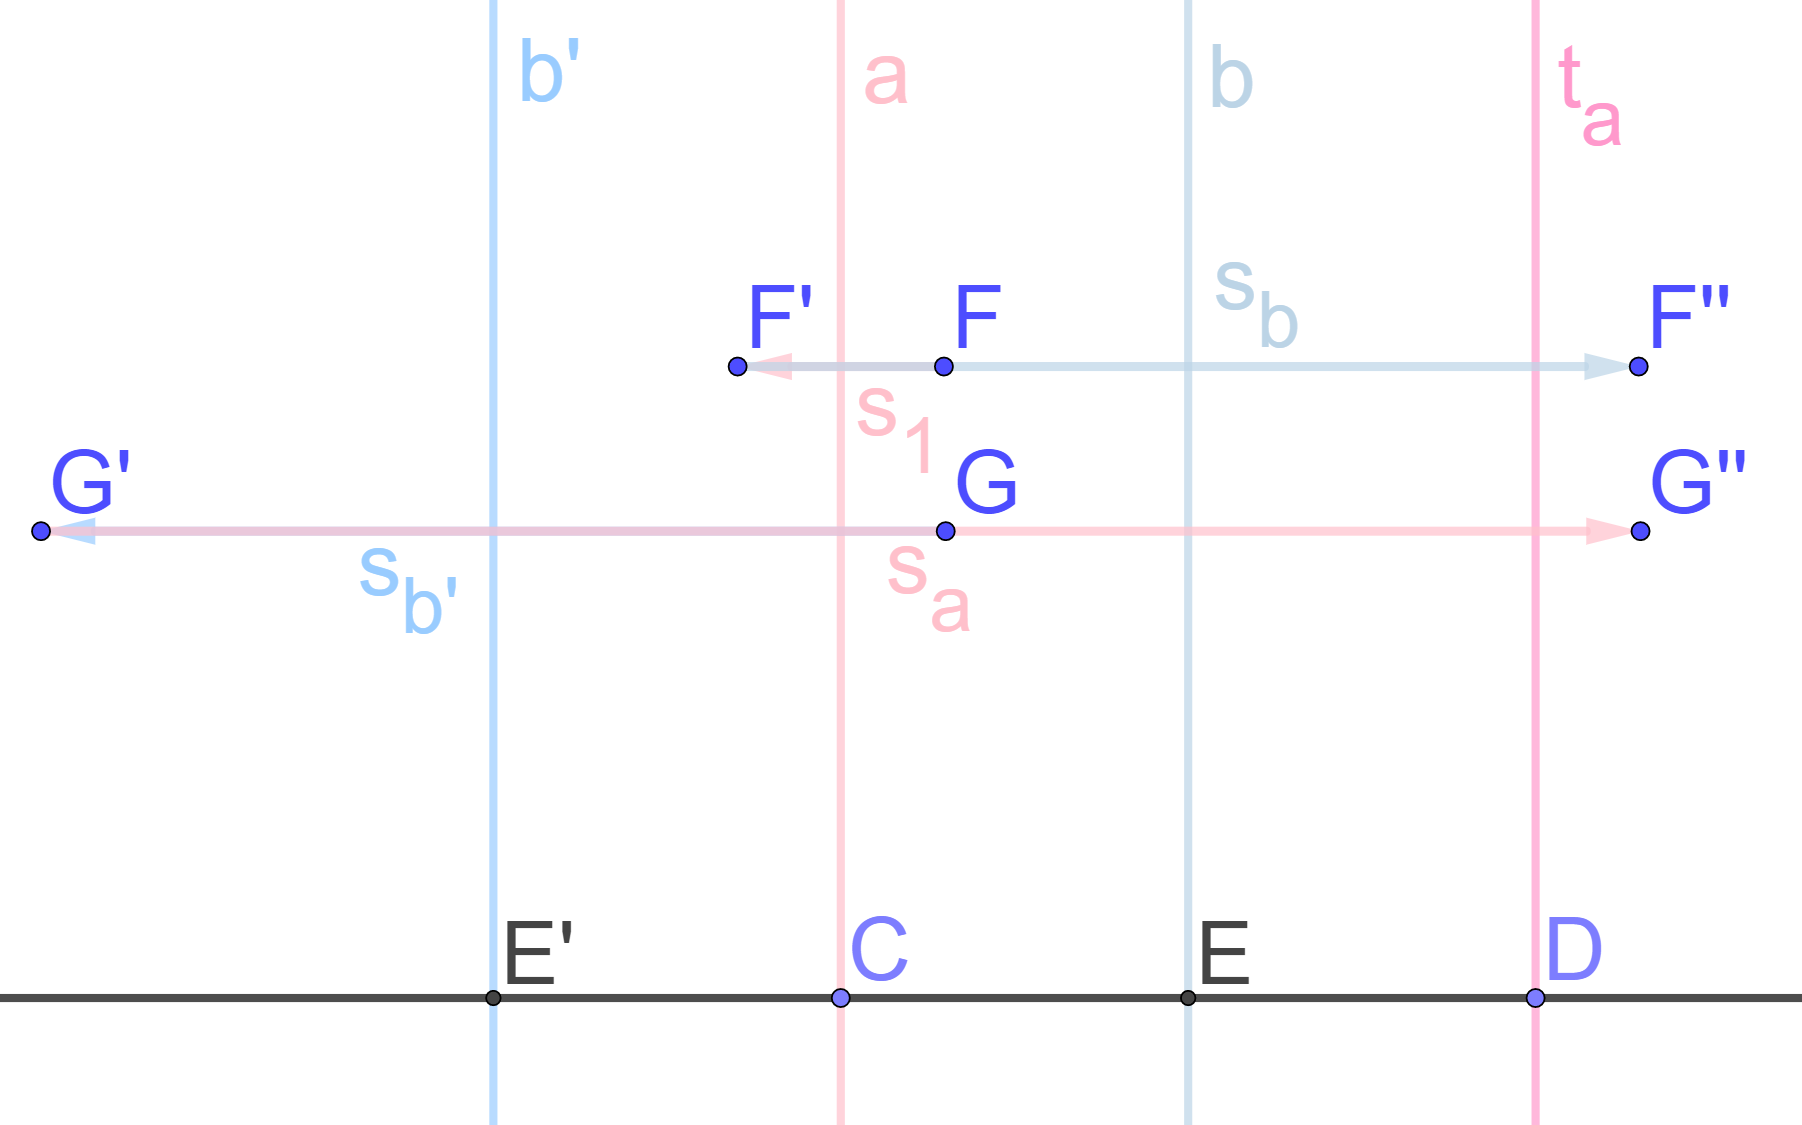
\includegraphics[width=7cm]{figuras/3-1.png}
	\vspace{-1em}
\end{figure}

\ej{3.2} Si $\pazocal{R}_P(\P) = \{g\in \iso(\P) \;|\; g \text{ es} $ 
	\linebreak
	rotación de centro $ P \} \cup \{ \text{id}_\P \}$ entonces
	\begin{itemizex}
		\item Si $a$ es una recta que pasa por $P$, entonces $g^{-1} = \sigma_a g \sigma_a$.
		\item $gh = hg$ para todo $g,h \in \pazocal{R}_P(\P)$.
		\item Para $X \in \P - \{P\}$ y $g(X) = h(X)$ entonces $g = h$.
	\end{itemizex}

\ej{3.3} Si $h$ es una isometría
 	\begin{itemizex}
 	\item Si $g \in \pazocal{R}_P(\P)$ entonces $hgh^{-1} \in \pazocal{R}_{h(P)}(\P)$
 	\item Si $r$ es una recta entonces $h\sigma_rh^{-1} = \sigma_{h(r)}$
	\end{itemizex}

\ej{3.3} Si $a, b$ son rectas en $\P$
	\begin{itemizex}
	 	\item $\sigma_a\sigma_b\sigma_a = \sigma_{a(b)}$
	 	\item $\sigma_a\sigma_b = \sigma_b\sigma_a \iff a \perp b$
	\end{itemizex}

\ejem{3.12} Sean $a,b$ tales que $a\perp_P b$. Entonces la rotación es de 180$^\circ$ y se
llama \textbf{reflexión central} si se denota como $\sigma_P$. Cumple las siguientes propiedades.
	\begin{itemizex}
		\item $\sigma_P\sigma_P= \text{id}_\P$
		\item Para todo $X$, $\sigma_P(X)$ es el único punto que cumple $P = \m[X, \sigma_P(X)]$.
		\item $\sigma_P$ es independiente de la elección de rectas $a\perp b$.
	\end{itemizex}

\tma{3.13} Las rectas $r$ y $\sigma_P(r)$ son paralelas.

\ejem{3.14} Una \textbf{reflexión con deslizamiento} $\phi$ es una composición de una reflexión $\sigma_c$ y una traslación $\tau$: $\phi = \tau\sigma_c$. $\phi$ deja invariante sólo la recta $c$, y no tiene ningún punto invariante.

\tma{3.15} Una isometría solo puede pertenecer a una de las de la tabla, y es una combinación de un número par o impar de reflexiones $\sigma$:

\begin{tabular}{l c c}
	& Con puntos fijos & Sin puntos fijos\\
	par & $\rho$ & $\tau$\\
	impar & $\sigma$ & $\phi$ \\
\end{tabular}


\tma{3.16} Si $g, g'$ son isometrías conjugadas, tienen la misma paridad.






	 
	 \end{multicols*}\pagebreak
	
	
	\begin{multicols*}{2}
	[\section{Ángulos}]
	\defi{4.1} Sean $r,l$ dos rectas con un punto $V$ en común. Sean $\overline{r}$ y $\overline{l}$ dos semirrectas determinadas por $V$ en $r$ y $l$. El par $\{\overline{l}, \overline{r} \}$ es un \textbf{ángulo}. $V$ es el vértice del ángulo y $\overline{l}$ y $\overline{r}$ son los lados del ángulo. El ángulo se designa por $\angle \{\overline{l}, \overline{r} \}$ o, si no hay lugar a confusión, $\angle V$. Así, por ejemplo, dado un triángulo $\triangle PQR$, $\angle P$ es el ángulo formado por $P$ con $[P,Q]$ y $[P,R]$.

\obs{4.4} Si $r = l$, y $\overline{r}_1$ y $\overline{r}_2$ son las semirrectas determinadas por $V$, entonces, en estas circunstancias, el ángulo $\angle\{ \overline{r}_1, \overline{r}_2 \}$ se denomina \textbf{ángulo llano} y $\angle\{ \overline{r}_1, \overline{r}_1 \}$ se denomina \textbf{ángulo nulo}.

\defi{4.5} Un ángulo $\angle \{\overline{l}, \overline{r} \}$ y un ángulo $\angle \{\overline{l}', \overline{r}' \}$ son \textbf{congruentes} si existe una isometría $g$ tal que $g(\{\overline{l}, \overline{r} \}) = \{\overline{l}', \overline{r}'\} $. Todos los ángulos que son congruentes forman una \textbf{clase de congruencia} de ángulos. Empleando la notación de vértices, la congruencia se denota como $\angle A = \angle B$.

\obs{4.6/4.8} Si  $\angle \{\overline{l}, \overline{r} \}$ tiene vértice $V$ y  $\angle \{\overline{l}', \overline{r}' \}$ tiene vértice $V'$, y $g$ es una isometría tal que $g(  \{\overline{l}, \overline{r} \}) =   \{\overline{l}', \overline{r}' \}$, entonces $g(V) = V'$. Asimismo, si existe una isometría $h$ que hace $h(V) = V'$, entonces  $h(  \{\overline{l}, \overline{r} \}) =   \{\overline{l}', \overline{r}' \}$.

\ejem{4.9} Consideramos las rectas $a \neq b$ que cortan en $V$, con sus respectivas semirrectas 
$\overline{a}_1, \overline{a}_2, \overline{b}_1, \overline{b}_2$. Consideramos $\angle \{\overline{a}_1, \overline{b}_1 \}$ y elegimos los puntos $A \in \overline{a}_1, B \in \overline{b}_1$ a igual distancia, $d(V,A) = d(V,B)$. Existe una recta $l \perp r_{AB}$ que pasa por $V$ (\tma{2.25/2.29}, que denominamos \textbf{bisectriz}. La bisectriz $l$ cumple que $\sigma_l(A) = B, \sigma_l(\overline{a}_1) = \overline{b}_1$ y viceversa. Además, si $\overline{l}$ es la semirrecta que corta a $[A,B]$, entonces $\angle \{\overline{a}_1, \overline{l} \} = \angle \{\overline{b}_1, \overline{l} \}$.

\tma{4.11} 

	 
	 \end{multicols*}\pagebreak
	
		
	\begin{multicols*}{2}
	[\section{Teorema de Tales}]
	\defi{5.0} Un \textbf{cuadrilátero} es una cuaterna ordenada de puntos [vértices] de $\P$, $(P, Q, R, S)$ formada por los segmentos $[P,Q], [Q,R], [R,S], [S,P]$ [lados] si dos cualesquiera segmentos son disjuntos o tienen un extremo en común. Dos vértices extremos del mismo lado son adyacentes y, si no, son opuestos.

\defi{5.1} Un cuadrilátero $\square PABC$ es un \textbf{paralelogramo} si $\m[P,B] = \m[A,C] = M$, donde los segmentos $[P,B]$ y $[A,C]$ son las diagonales, y $M$ es el centro.

\obs{5.2} Sea $\square PABC$ con centro $M$. Por las propiedades de las reflexiones centrales, se tiene que $\sigma_M(P) = B$ y $\sigma_M(A) = C$ [y viceversa]. Además, por tales propiedades, se tiene que $r_{PA} \parallel r_{BC}$ y $r_{PC} \parallel r_{AB}$; y $d(P,A) = d(B, C)$ y $d(P,C) = d(A,B)$. 

\obs{5.3} Si existen tres puntos $P,A,C$ no alineados, se puede construir un paralelogramo de varias maneras. Una forma es aplicar el axioma de las paralelas y proyectar $r_{PA}$ en $C$, y $r_{PC}$ en $A$. Otra forma es obtener $M  = \m[C,A]$, crear la recta $r_{PM}$ y proyectar el punto $B$ como el que $PM = d(P,M) = d(M,B) = MB$.

\obligatorio\tma{5.5 [Tales]} Sea $\triangle PAB$ y sean $A' \in [P,A]$, $B' \in  [P,B]$ dos puntos tales que $r_{AB} \parallel r_{A'B'}$. En estas condiciones se tiene que $\frac{PA'}{PA} = \frac{PB'}{PB}$.

\begin{figure}[H]
	\centering
	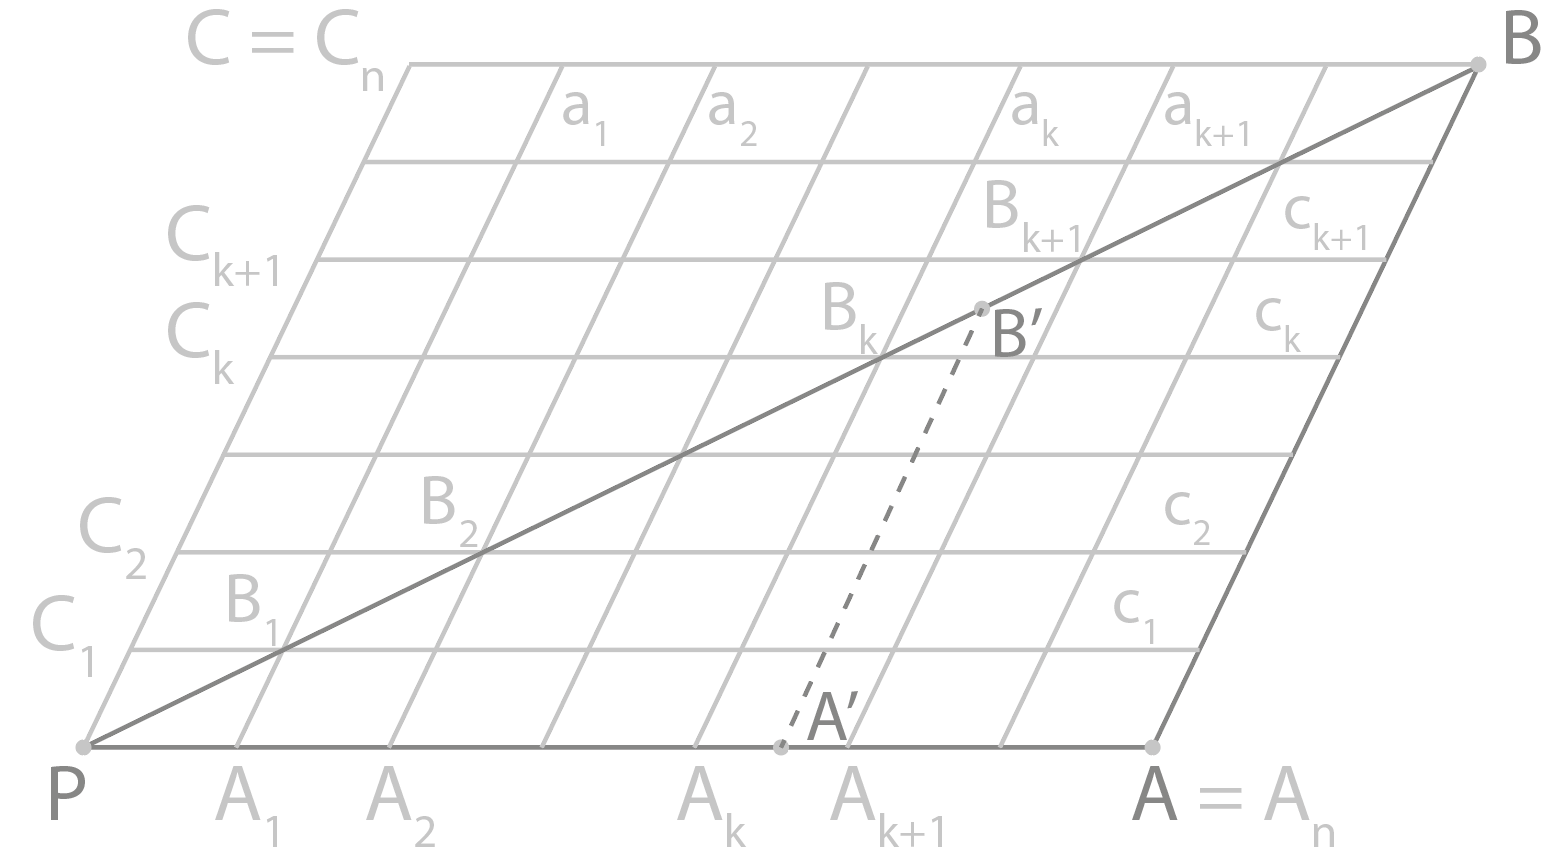
\includegraphics[width=8.2cm]{figuras/5-5.png}
	\vspace{-1em}
\end{figure}

\dem{Vamos a basar la demostración en la figura de arriba. 
Diseñamos el paralelogramo $\square PABC$ y dividimos el lado $[P,A]$ en $n$ segmentos con puntos de división $A_1, A_2, \cdots, A_n$, de modo que $d(A_i,A_{i+1}) = \frac{d(P,A)}{n}$. El mismo proceso se realiza con el lado $[P,C]$. Además, introducimos las rectas $a_k\parallel r_{PC}$ y $c_k\parallel r_{PA}$, de modo que el punto $P_{kl}$ es la intersección de $a_k$ con $c_l$. Vemos que $B_i = P_{ii}$. También observamos que existen los paralelogramos $\square A_kA_{k+1}P_{k+1,l}P_{k,l}$ y $\square C_lC_{l+1}P_{k,l+1}P_{k,l}$, de modo que $P_{kl}P_{k+1,l} = \frac{PA}{n}$ y $P_{kl}P_{k,l+1} = \frac{PC}{n}$.\linebreak
Ahora consideramos $B_k$. Sabemos que $\sigma_{B_k}(r) \parallel r$, $\sigma_{B_k}(c_k) = c_k$ y $\sigma_{B_k}(P_{k-1,k}) = P_{k+1,k}$. También, como $a_{k-1} \parallel a_{k+1}$, $\sigma_{B_k}(a_{k-1}) = a_{k+1}$, y por el mismo criterio, $\sigma_{B_k}(c_{k-1}) = c_{k+1}$. Con esto demostramos que $$\sigma_{B_k}(B_{k-1}) =\sigma_{B_k}(P_{k-1, k-1}) = P_{k+1, k+1}= B_{k+1}$$
Por tanto, los puntos $B_{k-1}, B_k, B_{k+1}$ están alineados y $B_{k-1}B_k = B_kB_{k+1}$. Por tanto, $B_kB_{k+1} = \frac{PB}{n}$.\linebreak
Es decir, hemos demostrado que
$$P_{kl}P_{k+1,l} = \frac{PA}{n} \quad  P_{kl}P_{k,l+1} = \frac{PC}{n} \quad P_{kl}P_{k+1,l+1} =  \frac{PB}{n}$$
Si reordenamos, tenemos que 
$$\frac{PA_k}{PA} = \frac{P_{0,0}P_{k,0}}{PA} = \frac{k}{n} = \frac{P_{0,0}P_{k,k}}{PB} =  \frac{PB_k}{PB}$$
Y con esto demostramos el teorema para los puntos $k$. Si tenemos $A'$ y $B'$ en la figura tales que $A' \in [A_k, A_{k+1}]$, de modo que $a' = r_{A'B'}$ está entre $a_k$ y $a_{k+1}$, y es paralelo a estas, haciendo que $B' \in [B_k, B_{k+1}]$. Por ser $A' \in [A_k, A_{k+1}]$ entonces $\frac{PA_k}{PA} \le \frac{PA'}{PA} \le \frac{PA_k}{PA}+\frac{1}{n}$ y, como $\frac{PA_k}{PA} = \frac{PB_k}{PB}$, entonces $\frac{PB_k}{PB} \le \frac{PA'}{PA} \le \frac{PB_k}{PB}+\frac{1}{n}$. Dado que $B'\in [B_k,B_{k+1}]$ entonces
$$\textcolor{SkyBlue}{\frac{PB'}{PB}-\frac{1}{n}} \le \frac{PB_k}{PB} \le \textcolor{SkyBlue}{\frac{PA'}{PA}} \le \frac{PB_k}{PB}+\frac{1}{n} \le \textcolor{SkyBlue}{\frac{PB'}{PB}+\frac{1}{n}}$$ 
Si nos fijamos en los elementos de azul, vemos que $n$ puede hacerse tan pequeño como queramos, de modo que, en el límite
$$\frac{PB'}{PB} \le \frac{PA'}{PA} \le \frac{PB'}{PB} \iff \frac{PB'}{PB} = \frac{PA'}{PA}$$ }

\cor{5.6} En base al teorema de Tales, se tiene que 
$$\frac{PA'}{PA} = \frac{PB'}{PB} = \frac{A'B'}{AB}$$

\defi{5.7} Dado un triángulo rectángulo $\triangle PAB$ con $\angle A$ recto, entonces la \textbf{hipotenusa} es el lado opuesto a $\angle A$, $[P,B]$. Los lados adyacentes, $[P,A],[B,A]$, son los \textbf{catetos}.
\begin{figure}[H]
	\centering
	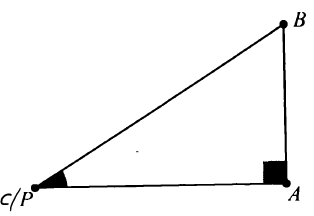
\includegraphics[width=3.5cm]{figuras/5-7.png}
	\vspace{-1em}
\end{figure}
\defi{5.8} Sea el triángulo rectángulo $\triangle PAB$ con $\angle A$ recto, entonces se definen las relaciones 
\begin{itemize}
	\item seno: $\text{sen}\angle P = \frac{BA}{PB}$
	\item coseno: $\text{cos}\angle P = \frac{PA}{PB}$
	\item tangente: $\text{tan}\angle P = \frac{BA}{PA}$
	\item cotangente: $\text{cot}\angle P = \frac{PA}{BA}$
\end{itemize}
\tma{5.10} Las razones trigonométricas para $\angle P$ no dependen del triángulo $\triangle PAB$, sólo de la clase de congruencia de $\angle P$.

\tma{5.12} Dado un triángulo rectángulo $\triangle ABC$ con $\angle A$ recto, la medida de los catetos, $AB,AC$, es menor que la de la hipotenusa $BC$.
\begin{figure}[H]
	\centering
	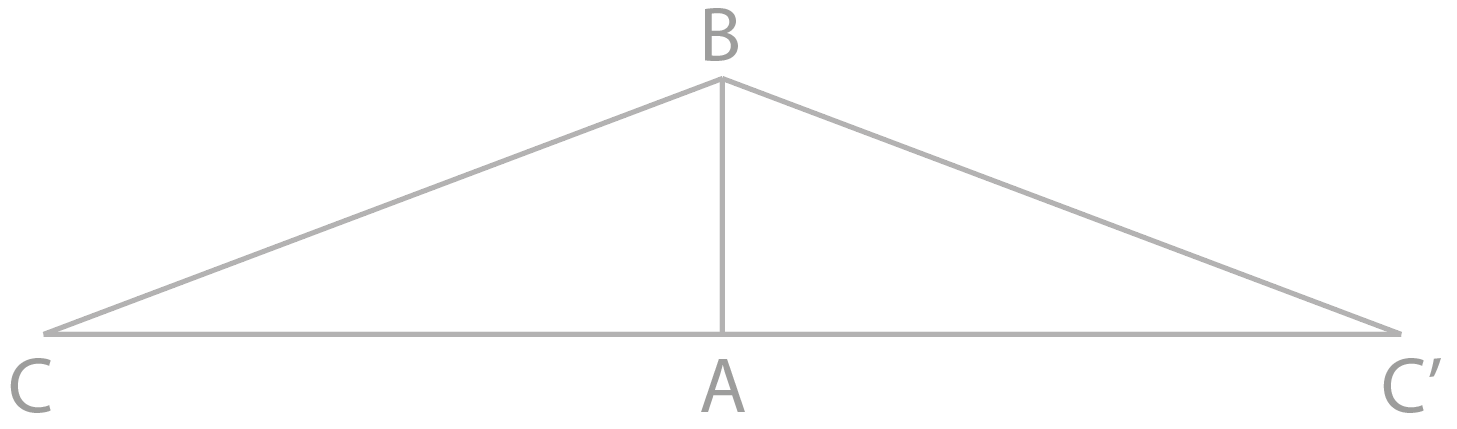
\includegraphics[width=6.5cm]{figuras/5-12.png}
	\vspace{-1em}
\end{figure}
\dem{Con la construcción anterior, vemos que los puntos $B, C, C'$ no están alineados, pues $C \in r_{AC}$ y $r_{AB}\perp r_{AC}$. Por la desigualdad triangular tenemos que $2AC = CC' < BC+BC' = 2BC$.}

\defi{5.13} La \textbf{medida de un ángulo} agudo $\angle P$ es el número real:
$$\measuredangle P = \arccos(\cos \angle P)$$
\tma{5.14 / 5.19} Si $\angle P = \angle Q$ entonces $\measuredangle P = \measuredangle Q$, sean $\angle P $ y $\angle Q$ agudos y obtusos.

\defi{5.15} Dado un ángulo $\angle{\overline{a}, \overline{b}_1} = \angle V$, un \textbf{ángulo suplementario} $\overline{\angle V} = \angle{\overline{a}, \overline{b}_2}$ es aquel donde $\overline{b}_1$ y $\overline{b}_2$ son las dos semirrectas de $b$ en $V$, y $\angle V$ y $\overline{\angle V}$ comparten $\overline{a}$. La suma de $\angle V$ y $\overline{\angle V}$ es un ángulo llano.

\tma{5.17} Si dos ángulos son congruentes, sus suplementarios lo son.

\defi{5.18} Para un ángulo obtuso $\angle P$ se tiene $\sen \angle P = \sen \overline{\angle P}$ y $\cos \angle P = -\cos \overline{\angle P}$

\end{multicols*}\pagebreak
	
	
	\begin{multicols*}{2}
	[\section{Teorema de Pitágoras}]
	\tma{6.1 [Pitágoras]} Para todo triángulo rectángulo $\angle ABC$ con $\angle A$ recto, se tiene que $$BC^2 = AC^2+ AC^2$$
\begin{figure}[H]
	\centering
	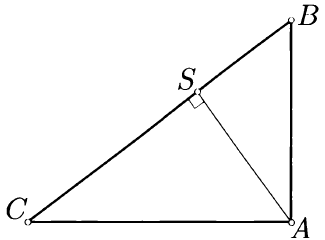
\includegraphics[width=3.5cm]{figuras/6-1.png}
	\vspace{-1em}
\end{figure}
\dem{Consideramos el punto $S\in r_{BC}$ tal que $r_{SA}\perp r_{CB}$. Pese a que es evidente, hay que demostrar que $S\in[B,C]$. Observamos que $SC < CA < BC$, la primera igualdad por $\cos \angle C = \frac{SC}{CA} < 1 \iff SC < CA$. Del mismo modo, $BS < BC$. Entonces, $S\in [B,C]$.\linebreak
Ahora observamos que
$$\cos \angle C = \frac{CA}{CB} = \frac{CS}{CA}$$
Por otra parte, también vemos que 
$$\cos \angle B = \frac{BS}{AB} = \frac{AB}{BC}$$
De ambas expresiones tenemos que (1) $CA^2 = CB\cdot CS$ y (2) $AB^2 = BS\cdot BC$. Así, $CB\cdot CS + CB\cdot BS = CB(CS+BS) = CB^2 = CA^2 + BA^2$.
}

\cor{6.3} Sea $\angle C$, entonces $$\sen^2 \angle C + \cos^2 \angle C = 1$$  

\dem{Si tenemos que $BC = 1$, entonces $\cos \angle C = \frac{CA}{CB}  = CA$ y $\sen \angle C = \frac{BA}{BC} = BC$. Aplicando el teorema de Pitágoras, entonces $ \sen^2 \angle C + \cos^2 \angle C =  BA^2 + CA^2 = BC^2 = 1$.} 

\tma{6.4} Dado $x \in [0, \pi] \subset \R$, existe un ángulo $\angle V$ tal que $\measuredangle V = x$.

\tma{6.5}  $\angle P = \angle Q$ sii $\measuredangle P = \measuredangle Q$

\defi{6.6} Sea $\triangle ABC$ y $h_B \perp r_{CA}$ y que pasa por $B$, y sea el punto $P_{h,b}$ el punto de corte de $h_B$ y $r_{CA}$. Entonces, $P_{h,b}$ es el \textbf{pie de la altura de $B$}, y $[P_{h,b},B]$ es la \textbf{altura} de $\triangle ABC$ desde $B$.
\begin{figure}[H]
	\centering
	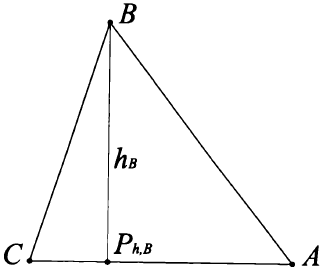
\includegraphics[width=3.5cm]{figuras/6-6.png}
	\vspace{-1em}
\end{figure}

\tma{6.7} En el triángulo de la \defi{6.6}, si $\angle A$ y $\angle C$ son agudos, entonces $P_{h,b} \in [C,A]$. Si $\angle A$ o $\angle C$ es obtuso, entonces $P_{h,b} \not\in [C,A]$.

\tma{6.8 [Fórmula del coseno]} Sea $\triangle ABC$ un triángulo, entonces se cumple que $$BC^2 = AB^2 + AC^2 - 2\cdot AB \cdot AC \cdot \cos \angle A$$
\dem{Basándonos en la figura de la \defi{6.6}, y por el \tma{6.7} [en el caso de $\triangle$ acutángulo], entonces se forman dos triángulos rectángulos $\triangle P_{hB}BC$ y $\triangle P_{hB}BA$ donde se verifica que $CA = CP_{hB} + P_{hB}A$
Por el \tma{de Pitágoras} tenemos que
$$AB^2 = P_{hB}A^2 + P_{hB}B^2 \qquad BC^2 = BP_{hB}^2+P_{hB}C^2$$
Si sustituimos una igualdad en otra tenemos que 
$$BC^2 = CP_{hB}^2 + AB^2 - P_{hB}A^2$$
Como $CA = CP_{hB} + P_{hB}A$ entonces
$$BC^2 = (CA - P_{hB}A)^2 + AB^2 - P_{hB}A^2 = $$
$$CA^2  \textcolor{SkyBlue}{+P_{hB}A^2} - 2\cdot CA\cdot P_{hB}A  + AB^2  \textcolor{SkyBlue}{-P_{hB}A^2}$$
Si quitamos las partes en azul, y consideramos que $P_{hB}A = AB\cos\angle A$, entonces queda el teorema demostrado.}

\cor{6.9} Dado un triángulo donde $BC^2 = AB^2 + AC^2$ entonces es un triángulo rectángulo, con $\angle A$ recto. 
\dem{Si aplicamos el \tma{del coseno}, entonces, el término $ 2\cdot AB \cdot AC \cdot \cos \angle A = 0$, y como $AB \neq 0, AC \neq 0$, entonces $\cos \angle A = 0 \iff \angle A$ es recto (\tma{6.5}).} 

\tma{6.10 [Fórmula de los senos]} Sea $\triangle ABC$, entones se verifica
$$\frac{AB}{\sen \angle C} = \frac{AC}{\sen \angle B}  = \frac{BC}{\sen \angle A}$$
\dem{Seguimos con la figura de la \defi{6.6}. Vemos que $BP_{hB} = BC\sen \angle C = BA\sen\angle A$. Si el triángulo es obtusángulo también se cumple porque los senos se mantienen.
Simplemente, igualando $BP_{hB}$ tenemos que $\frac{BC}{\sen \angle A} = \frac{BA}{\sen \angle C}$. El resto de igualdades se consiguen con las demás alturas.}





\end{multicols*}\pagebreak
	

	\begin{multicols*}{2}
	[\section{Semejanzas}]
	\defi{7.1} Sea $C$ un punto de $\P$ y $k > 0$. Una \textbf{homotecia} $\eta_{C,k}:\P \rightarrow \P$ es una aplicación tal que a cada punto $P \in r_{CP}$ le hace corresponder un punto $\eta_{C,k}(P) \in r_{CP}$ tal que $C\eta_{C,k}(P) = kCP$. $k$ es la \textbf{razón de homotecia}.

\obs{7.2} Sea $X \in \P$, $\eta_{C,k}$ y $\gamma$ una aplicación del \axioma{P3}. Entonces se cumple que $\gamma(\eta_{C,k}(X)) = \gamma(C) + k(\gamma(X)-\gamma(C))$

\obs{7.3} Toda homotecia es una biyección que tiene
\begin{itemizex}
	\item Identidad: $\eta_{C,1}$
	\item Inversa: $\eta_{C,1/k}$
\end{itemizex}

\tma{7.4}/\cor{7.5} Sean $A, B$ y $\eta_{C,k}$, entonces $\eta_{C,k}(A)\eta_{C,k}(B) = kAB$. Además, $\eta_{C,k}[A,B] = [\eta_{C,k}(A), \eta_{C,k}(B)]$.

\tma{7.7} Toda homotecia envía un ángulo a un ángulo congruente, y toda recta a una paralela.

\defi{7.8} Una \textbf{semejanza} es una combinación de homotecias e isometrías.

\cor{7.10/7.11} / \tma{7.19} Toda semejanza envía rectas a rectas, segmentos a segmentos, y conserva los ángulos. Toda biyección $\psi$ que cumpla estas condiciones es una semejanza.

\tma{7.12} / \cor{7.13} Toda semejanza $\delta$ cumple que $\delta(A)\delta(B) = kAB$, donde $k$ es la razón de semejanza. Dados $A,B,C,D$, entonces se cumple que 
$$\frac{AB}{CD} = \frac{\delta(A)\delta(B)}{\delta(C)\delta(D)}$$

\tma{7.15} Si $\angle A = \angle B$, entonces existe $\delta$ tal que $\delta(\angle A) = \angle B$.

\tma{7.18} Sean $\triangle ABC$ y $\triangle AB'C'$ que comparten $\angle A$ y $A,B,B'$ están alineados, así como $A, C, C'$. Entonces si existe $k$ tal que $AB' = kAB$ y $AC' = kAC$ entonces $\triangle ABC$ y $\triangle AB'C'$ son semejantes, $r_{BC} \parallel r_{B'C'}$ y $B'C' = kBC$.

\defi{7.20} Se llama \textbf{mediana} al segmento que une cada vértice con el punto medio del lado opuesto de un triángulo. Es decir, dado $\triangle ABC$, las medianas son $[A, \m[B,C]]$, $[B, \m[A,C]]$ y $[C, \m[A,B]]$.

\tma{7.21} Las tres medianas de un triángulo cortan en un punto $G$, llamado \textbf{baricentro}.
\begin{figure}[H]
	\centering
	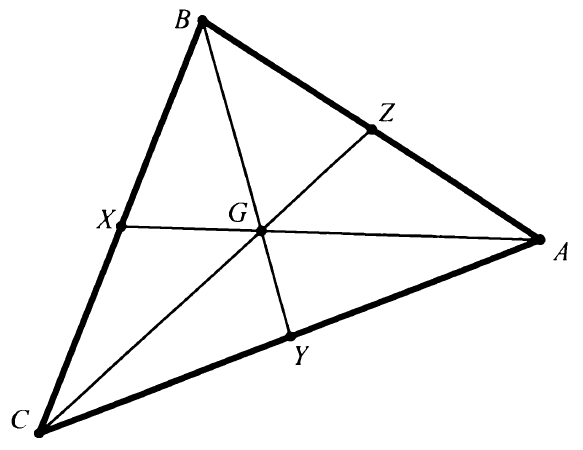
\includegraphics[width=5.5cm]{figuras/7-21.png}
	\vspace{-1em}
\end{figure}
\obligatorio\dem{Definimos $X = \m[B,C], Y = \m[A,C], Z = \m[A,B]$ y sea $G$ $[B,Y] \cap [C,Z]$. El punto existe porque, si definimos la recta $r_{BY}$, entonces $C$ está en uno de los semiplanos de la recta (pongamos, $H^2$) y, si $A \in H^1$, entonces $Z \in H^1$, $C$ y $Z$ están en distintos semiplanos de $r_BC$.
Si tomamos $\triangle ABC$ y $\triangle AZY$ entonces, por ser $Y,Z$ puntos medios, entonces, por el \tma{7.18}, $r_{YZ} \parallel r_{BC}$ y $BC = 2YZ$. Además, por ser los ángulos entre $[C,Z]$ y $[B,Y]$ alternos internos, los triángulos $\triangle GYZ$ y $\triangle GBC$ son semejantes de razón $2$. Por tanto, $GB = 2GY$ y $GC = 2GZ$.
Si repetimos esto con $[A,X]$ y $[B,Y]$, entonces existe un punto $G'$ tal que $G'A = 2G'X$ y $G'B = 2G'Y$. Como $\frac{G'B}{G'Y} = \frac{GB}{GY}$, entonces $G = G'$ y las tres medianas cortan en $G$. }

\tma{7.23} Las tres mediatrices de un tríangulo cortan en un punto, el \textbf{circuncentro}.
\begin{figure}[H]
	\centering
	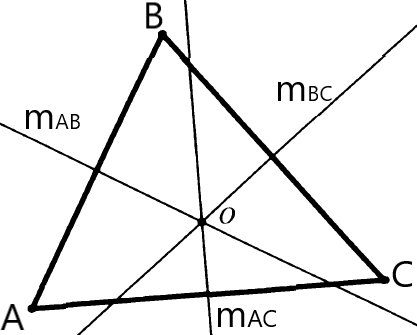
\includegraphics[width=4.5cm]{figuras/7-23.png}
	\vspace{-1em}
\end{figure}
\obligatorio\dem{Si $\triangle ABC$ es un triángulo, las mediatrices $m_{AB}$ y $m_{BC}$ cortan en un punto $O$. Si no cortaran, entonces $m_{AB} \parallel m_{BC}$, y como $r_{AB}\perp m_{AB}$ y $m_{BC} \perp r_{BC}$ entonces $r_{AB} \parallel r_{BC}$, lo cual es absurdo. Por ser $m_{BC}$ mediatriz, entonces $OB = OC$, y $OA = OB$ para $m_{AB}$. Entonces $OA = OC$ y por tanto $O \in m_{AC}$, luego $O$ corta las tres mediatrices.  }

\tma{7.24} Las tres alturas de un triángulo se cortan en el \textbf{ortocentro}
\begin{figure}[H]
	\centering
	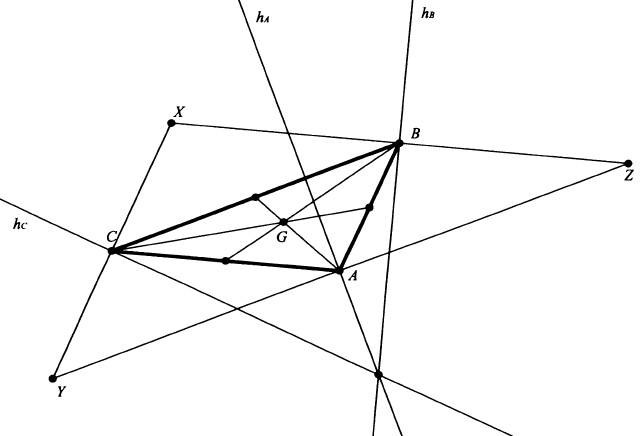
\includegraphics[width=8.5cm]{figuras/7-24.png}
	\vspace{-1em}
\end{figure}
\obligatorio\dem{Sea $\triangle ABC$ el triángulo con baricentro $G$ y sean $h_A, h_B, h_C$ sus alturas. Consideramos la semejanza $\tau = \sigma_G \eta_{G,2}$, de modo que $\triangle ABC$ se transforma en $\triangle XYZ$, con $\tau(A) = X, \tau(B) = Y, \tau(C) = Z$. Por las propiedades de las semejanzas, $r_{BC} \parallel r_{YZ}, r_{AC} = r_{XZ}, r_{AB} \parallel r_{XY}$, y se cumple que $A = \m[Y,Z], B=\m[X,Z], C = \m[X,Y]$. Por tanto, ahora $h_A = m_{YZ}, h_B = m_{XZ}, h_C = m_{XY}$ y, por tanto, el ortocentro de $\triangle ABC$ es el circuncentro de $\triangle XYZ$.}

\tma{7.25 [Recta de Euler]} 
Dado un triángulo, su baricentro $G$, ortocentro $O$ y circuncentro $H$ pertenecen a una misma recta (si el triángulo no es equilátero). Además, $OH = 2OG$.

\obligatorio\dem{Si partimos del triánguo con baricentro $G$ y aplicamos la semejanza $\tau = \sigma_G\eta_{G,2}$, como en el \tma{7.24}, entonces se cumple que $\tau(O) = H$. Por ser $\sigma_G$, entonces $H\in r_{OG}$ y por ser $\eta_{G,2}$, entonces $OH = 2OG$.}

\cor{7.26} El \textbf{incentro} del triángulo es el punto donde se cortan las tres bisectrices del triángulo.

\ej{7.7 [Teorema de Ceva]} En $\triangle ABC$ sean $X \in [B,C], Y \in [C,A], Z \in [A,B]$. Si $X,Y,Z$ no coinciden con ninguno de los vértices del triángulo, entonces los segmentos $[A,X],[B,Y],[C,Z]$ se cortan en un punto sii
$$\frac{AZ}{ZB}\frac{BX}{XC}\frac{CY}{YA} = 1$$

\ej{7.8 [Teorema de Menelao]} Sea $\triangle ABC$ y sean $X \in r_{BC}, Y \in r_{CA}, Z \in r_{AB}$. Entonces, sii $X,Y,Z$ están alineados se cumple que 
$$\frac{AZ}{ZB}\frac{BX}{XC}\frac{CY}{YA} = 1$$








\end{multicols*}\pagebreak
	
	\begin{multicols*}{2}
	[\section{Circunferencias}]
	\defi{8.1} Sea $O \in \P$ y $\rho > 0$. Entonces una \textbf{circunferencia} $\C$ es el conjunto de puntos a una distancia $\rho$ de $O$. $O$ es el \textbf{centro} y $\rho$ el \textbf{radio}.

\tma{8.3} Una circunferencia corta a una recta en a lo sumo dos puntos.

\defi{8.4} Dada $\C$ una recta que corta en dos puntos se llama \textbf{secante}, que corta en un punto se llama \textbf{tangente} y que no corta se llama \textbf{exterior}. Si para un punto $X \in \P, d(O,X) > d(O,\rho)$ el punto es exterior, y si $d(O,X) < d(O, \rho)$ entonces es interior.

\tma{8.5} Sea $\C$ con centro $O$. Si $t$ es tangente a $\C$ en $P_t$, entonces $t \perp r_{O,P_t}$.

\defi{8.6} Sean $P, P'$ dos puntos tales que $O =  \m[P,P']$. Entonces, si los puntos están en $\C$, se denominan \textbf{diametralmente opuestos en $\C$}, y $[P,P']$ es un diámetro de $\C$.

\tma{8.7}/\defi{8.9} Dados tres puntos no alineados, entonces existe una única circunferencia                                                                                                                                                                                                                                                                                                                                                                                                                                                                                                                                                                                                                                                                                                                                                                                                                                                                                                                                                                                                                                                                                                                                                                                                                                                                                                                                                                                                                                                                                                                                                                                                                                                                                                                                                                                                                                                                                                                                                                                                                                                                                                                                                                                                                                                                                                                                                                                                                                                                                                                                                                                                                                                                                                                                                                                                                                                                                                                                                                                                                                                                                                                                                                                                                                                                                                                                                                                                                                                                                                                                                                                                                                                                                                                                                                                                                                                                                                                                                                                                                                                                                                                                                                                                                                                                                                                                                                                                                                                                                                                                                                                                                                                                                                                                                                                                                                                                                                                                                                                                                                                                                                                                                                                                                                                                                                                                                                                                                                                                                                                                                                                                                                                                                                                                                                                                                                                                                                                                                                                                                                                                                                                                                                                                                                                                                                                                                                                                                                                                                                                                                                                                                                                                                                                                                                                                                                                                                                                                                                                                                                                                                                                                                                                                                                                                                                                                                                                                                                                                                                                                                                                                                                                                                                                                                                                                                                                                                                                                                                                                                                                                                                                                                                                                                                                                                                                                                                                                                                                                                                                       que pase por estos puntos, la \textbf{circunferencia circunscrita}.

\cor{8.8} Dos circunferencias tienen a lo sumo dos puntos en común. Si sólo tienen un punto en común se llaman \textbf{tangentes}.

\importante \tma{8.10} Sean $\C, \C'$ con centros $O, O'$ y radios $\rho, \rho'$ respectivamente. Si las dos circunferencias cortan en dos puntos, entonces se cumplen las siguientes desigualdades:
$$OO' < \rho+\rho' \quad \rho < OO'+\rho' \quad \rho' < OO' + \rho$$
Y si las circunferencias son tangentes, entonces se verifica una de estas igualdades:
$$OO' = \rho+\rho' \quad \rho = OO'+\rho' \quad \rho' =   OO' + \rho$$      

\tma{8.11} Sea $\C$ con centro $O$ y sean $\triangle PXY$ y $\triangle P'XY$ dos triángulos con vértices en $\C$ y $P, P', O$ están en el mismo semiplano determinado por $r_{XY}$. Si $X$ e $Y$ no son diametralmente opuestos, entonces $\measuredangle P = \measuredangle P' = \frac{1}{2}\measuredangle O$
\begin{figure}[H]
	\centering
	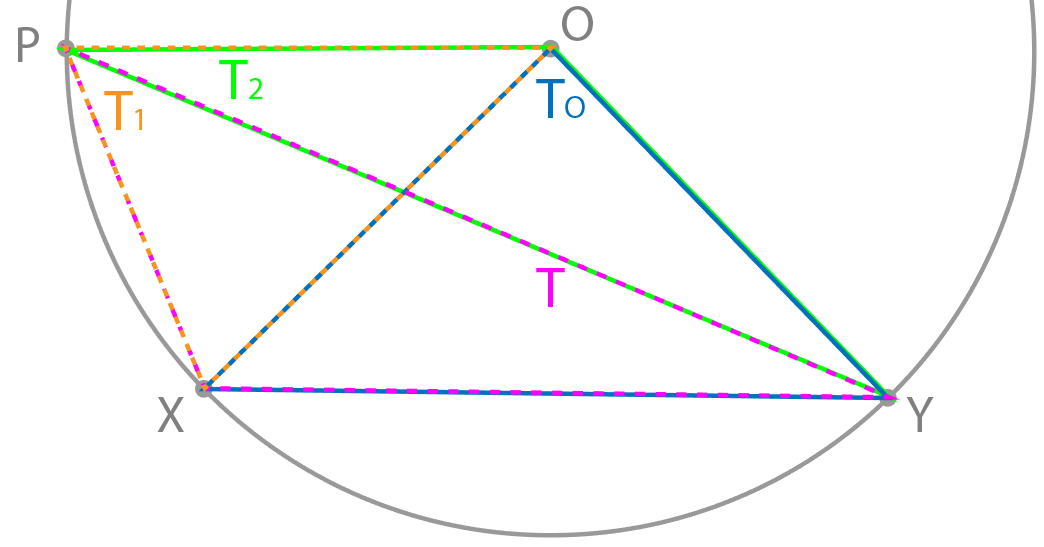
\includegraphics[width=7.5cm]{figuras/8-10.png}
	\vspace{-1em}
\end{figure}
\obligatorio\dem{Sea $\pazocal{T} = \triangle PXY$ y $\pazocal{T}_O =\triangle OXY$. Construimos también $\pazocal{T}_1 = \triangle POX$ y $\pazocal T_2 = \triangle POY$, isósceles, de modo que $\measuredangle_{\pazocal{T}_1} X = \measuredangle_{\pazocal{T}_1} P $ y $\measuredangle_{\pazocal{T}_2} Y = \measuredangle_{\pazocal{T}_2} P$. Como la suma de los ángulos de $\pazocal{T}_1$ y $\pazocal{T}_2$ es llano, entonces
$$2\measuredangle_{\pazocal{T}_1} P = \pi - \measuredangle_{\pazocal{T}_1} O \qquad 2\measuredangle_{\pazocal{T}_2} P = \pi - \measuredangle_{\pazocal{T}_2} O$$
Vamos a suponer ahora que $\measuredangle_{\pazocal{T}} P = \measuredangle_{\pazocal{T}_1} P-\measuredangle_{\pazocal{T}_2} P$. Para $2\measuredangle_{\pazocal{T}} P$ entonces se cumple que 
$$2\measuredangle_{\pazocal{T}} P = 2\measuredangle_{\pazocal{T}_1} P-2\measuredangle_{\pazocal{T}_2} P = \measuredangle_{\pazocal{T}_2}O-\measuredangle_{\pazocal{T}_1} O = \measuredangle_{\pazocal{T}_O} O = \measuredangle O$$
La misma demostración sucede para  $\measuredangle_{\pazocal{T}} P = \measuredangle_{\pazocal{T}_1} P+\measuredangle_{\pazocal{T}_2} P$ y  $\measuredangle_{\pazocal{T}} P = \measuredangle_{\pazocal{T}_2} P-\measuredangle_{\pazocal{T}_1} P$
} 

\defi{8.13} Sea $\C$ con centro $O$ y radio $\rho$. Se denomina \textbf{inversión} del plano con respecto a $\C$ a una aplicación $\iota_\C: \P- \{O\}\rightarrow \P-\{O\}$ que a cada punto $P$ le hace corresponder otro punto $\iota_\C(P)$ tal que $O, P, \iota_\C(P)$ están alineados, $O\not\in [P, \iota_\C(P)]$ y se verifica que 
$$OP\cdot O_{\iota_\C}(P) = \rho^2$$
Esta aplicación verifica que 
\begin{itemizex}
	\item $\iota_\C\circ \iota_\C(P) = P$ para todo $P\in \P -{O}$.
	\item Para todo $P \in \C$ se cumple $\iota_\C(P) = P$. A todo punto fuera del circulo, $\iota_\C$ lo manda dentro, y viceversa.
	\item Si $r$ pasa por $O$, $\iota_\C(r-\{O\}) = r-\{O\}$.
\end{itemizex}
\begin{figure}[H]
	\centering
	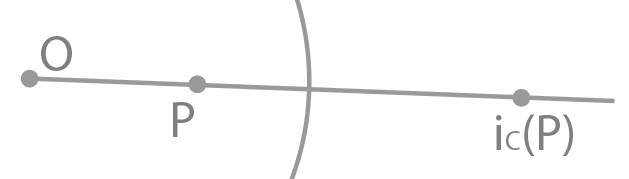
\includegraphics[width=7.5cm]{figuras/8-15.png}
	\vspace{-1em}
\end{figure}
\tma{8.16/8.17} Sea $\C$ y $P\in \P$. Sean $a, b$ rectas que cortan a $P$ y secantes a $\C$. Sean $A_1$ y $A_2$ los puntos de corte de $a$ con $\C$ y $B_1, B_2$ los de $b$ con $\C$. Entonces se verifica que 
\[PA_1\cdot PA_2 = PB_1 \cdot PB_2  \] 
Si $a$ es tangente, entonces 
\[PA^2 = PB_1 \cdot PB_2  \] 
Ese producto, por tanto, es invariante de la recta, y se denomina \textbf{potencia de $P$ con respecto a $\C$}.

\tma{8.18} Sea $\C$ de radio $\rho$ y centro $O$.
\begin{itemizex}
	\item Sea $\C'$ una circunferencia de centro $O'$ que pasa por $O$, entonces $\iota_\C(\C'-\{O\})$ es una recta ortogonal a $r_{O,O'}$. Sea $r$ que no pasa por $O$, entonces $\iota_\C(r) = \C'-\{O\}$, donde $\C'$ es una circunferencia que pasa por $O$.
	\begin{figure}[H]
		\centering
		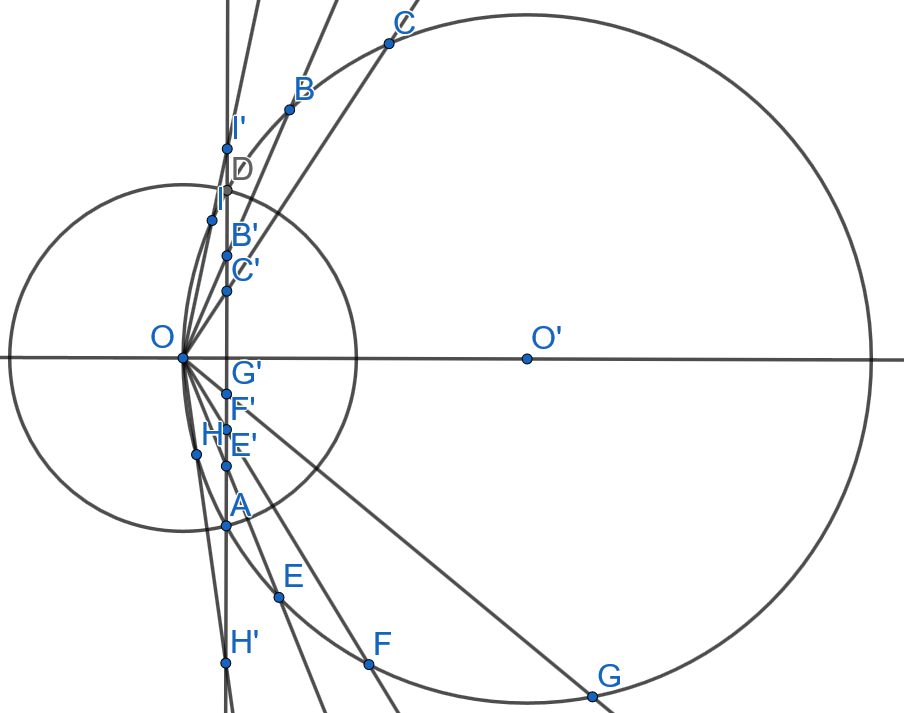
\includegraphics[width=7.5cm]{figuras/8-18-1.png}
		\vspace{-1em}
	\end{figure}
	\item Si $\C'$ no pasa por $O$ entonces $\iota_\C(\C')$ es otra circunferencia que no pasa por $O$. Si $O$ es exterior a $\C'$ entonces $\iota_\C(\C')$ es la imagen de $\C'$ por la homotecia de centro $O$ y razón $\rho^2/t$, donde $t$ es la potencia de $O$ con respecto a $\C'$. Si $O$ es interior a $\C'$ entonces $\iota_\C(\C') = \sigma_O \circ \eta_{O,\rho^2/t}(\C)$.
	\begin{figure}[H]
		\centering
		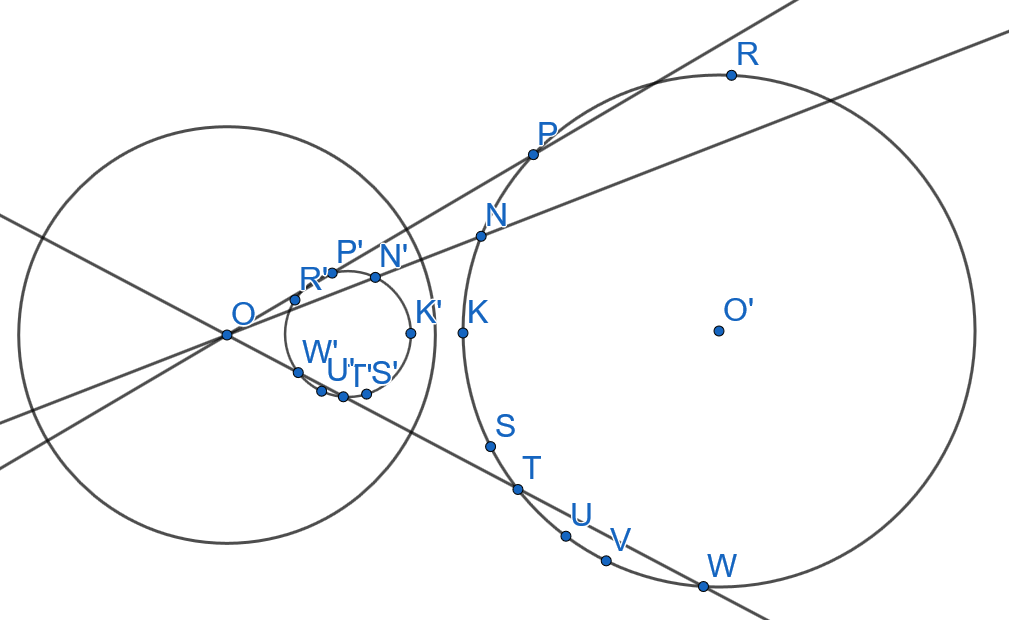
\includegraphics[width=7.5cm]{figuras/8-18-2.png}
		\vspace{-1em}
	\end{figure}
\end{itemizex}

\defi{8.19} Sea $A,B,C,D$ una cuaterna ordenada de puntos distintos del plano. Se define \textbf{razón doble} como 
$$(A,B:C,D) = \frac{CA}{CB}:\frac{DA}{DB}$$. 
Si $A,B,C,D$ están alineados, entonces la razón doble es una razón de las dos razones simples: $\frac{CA}{CB}\frac{DB}{DA}$.

Por convenio se tiene que 
$$(A,B:C,\infty) = \frac{CA}{CB}$$


\tma{8.20} Sea $\C$ con centro $O$ y sean $A,B \neq O$ 
y que no estén alineados a $O$. Si $\iota_\C(A)=A'$ y $\iota_\C(B) = B'$, los triángulos $\pazocal(T)_1 = \triangle OAB$ y $\pazocal (T)_2 = \triangle OA'B'$ son semejantes, y $\angle A = \angle B'$ y $\angle B = \angle A'$.

\tma{8.21} Sea $\C$ con centro $O$ y sean $A, B, C, D\neq O$. Entonces
$$(A,B:C,D) = (\iota_\C(A), \iota_\C(B):\iota_\C(C),\iota_\C(D))$$

\end{multicols*}\pagebreak
	
	\begin{multicols*}{2}
	[\section{Geometría hiperbólica}]
	\defi{9.0} Para describir la geometría hiperbólica se fija una recta $l_{\infty}$ y uno de los semiplanos de la recta $l_\infty$ como $\H$. La distancia hiperbólica sigue la lógica de para que dos pares de puntos $A, A'$ y $B,B'$ sobre $r\perp l_\infty$ y $d(A,A') = d(B,B')$, pero $A,A'$ están más cerca de $l_\infty$ que $B, B'$, entonces $d_\H(A,A') > d_\H(B,B')$.

Si $R = r\cap l_\infty$, definimos la \textbf{distancia hiperbólica} como
$$d_\H(P,Q) = \left| \log \frac{RP}{RQ} \right| = |\log(P,Q:R,\infty)| $$

\tma{9.1} Sean $P,Q,S$ en $\H$ sobre $r \perp l_\infty$ tal que $Q\in[P,S]$. Entonces:
\begin{itemizex}
	\item $d_H (P,Q) + d_H(Q,S) = d_H(P,S)$.
	\item Sea $\C$ con centro $R = r \perp l_\infty$, entonces
	$$d_H(\iota_\C(P), \iota_\C(Q)) = d_H(P,Q)$$
\end{itemizex}

\tma{9.2} Sean $P,Q \in \H$ de modo que $r_{PQ} \not\perp l_\infty$. Existe una única circunferencia $\C_{PQ}$ con centro $l_\infty$ y que pasa por $P$ y $Q$.

\defi{9.0-cont} Queremos que la distancia anterior sea invariante a inversiones respecto a circunferencias. 
Si tenemos  $P,Q \in \H$ de modo que $r_{PQ} \not\perp l_\infty$ y $X,Y = \C_{PQ}\cap l_\infty$, podemos crear $\C_X$. Entonces, se tiene que la recta $r_{\iota_{\C_X}(P)\iota_{\C_X}(Q)} \perp l_\infty$, y definimos 
$$d_H(P,Q) = d_H(\iota_\C(P), \iota_\C(Q)) = |\log(\iota_\C(P), \iota_\C(Q):R,\infty)|$$
Sin embargo, por el \tma{8.21} la razón doble conserva las inversiones, luego
$$|\log(\iota_\C(P), \iota_\C(Q):R,\infty)| =$$$$ |\log(\iota_\C\iota_\C(P), \iota_\C\iota_\C(Q):\iota_\C(R),\infty)| =$$
$$|\log(P, Q:\iota_\C(R),\iota_\C(\infty))|$$
Si tomamos como convención $\iota_\C(\infty) = X$, y por el \tma{8.18}, $\iota_\C(R) = Y$ entonces
$$d_H(P,Q) = |\log(P,Q:Y,X)|$$

\tma{9.3} Sea $\C$ con centro $l_\infty$, entonces $\iota_\C$ preserva las distancias hiperbólicas para todo $P,Q$:
$$d_H(P,Q) = d_H(\iota_\C(P), \iota_\C(Q))$$

\tma{9.4} Si $\C$ tiene centro en $l_\infty$, entonces $\C \cap H$ es una recta hiperbólica.

\defi{9.5} Dos rectas hiperbólicas son paralelas si son disjuntas o coinciden.

\tma{9.6} Sea $r_H$ hiperbólica y $P$ un punto de $\H$ que no está en $r_H$. Existen infinitas rectas hiperbólicas paralelas a $r_H$ que pasan por $P$.




 

\end{multicols*}\pagebreak
	
	\begin{multicols*}{2}
	[\section{Polígonos}]
	\defi{10.1} Un polígono $\PP$ es un conjunto finito
$\{\cdots, [V,W],\cdots \}$ de $r$ segmentos llamados lados del polígono. Los extremos de los lados, vértices, forman el conjunto $\{V_1,\cdots,V_r \}$. $\PP$ cumple
\begin{itemizex}
	\item Dos lados de $\PP$ o bien no se cortan o tienen únicamente un extremo común (son lados adyacentes).
	\item Los lados de $\PP$ pueden escribirse como una sucesión finita de vértices $[V_1,V_2],[V_2,V_3],\cdots,[V_r,V_1]$.
\end{itemizex}

\defi{10.4} Une \textbf{diagonal} es un segmento cuyos extremos son dos vértices que no pertenecen al mismo lado.

\defi{10.6} Sea $V$ un vértice de $\PP$ y sean $[V,W_1]$ y $[V,W_2]$ dos lados. El ángulo con vértice $V$ y semirrectas que contienen a ambos lados forman el ángulo $\angle V$ de $\PP$.

\defi{10.8} Un polígono es \textbf{convexo} si toda recta que no contiene a ninguno de los lados del polígono corta a lo sumo en dos lados de éste.

 \tma{10.10} Un polígono $\PP$ es convexo sii para todo lado $[V,W]$ de $\PP$ los vértices de $\PP$ distintos de $V$ y $W$ están todos en el mismo de los dos semiplanos determinados por $r_{VW}$.
 
 \defi{10.11} Un punto $P$ está en el \textbf{interior} de un polígono convexo $\PP$ si cualquier recta que pase por $P$ corta a los lados del polígono en dos puntos. Si $P$ no está ni en el interior ni en los lados del polígono, entonces está en el exterior. 
 
 \obs{10.12} Un punto $P$ está en el interior de un polígono $\PP$ si existe una recta $r$ que pasa por $P$ de modo que si $\overline{s}$ es una de las semirrectas, $\overline{s}$ corta a $\PP$ en un número $n$ impar de puntos que no son vértices.
 
 \defi{10.13} Un polígono convexo es \textbf{regular} si todos sus lados y ángulos son congruentes.
 
 \lema{10.14} Sean $r$ y $s$ rectas que al cortarse forman un ángulo $\pi/n$. Sean $\sigma_r$ y $\sigma_s$. Si $V$ es un punto en $r$, definimos los puntos $V_{i+1} = (\sigma_s \circ \sigma_r)^i(V), \quad i=1,\cdots, n-1$, es decir, las imágenes de $V$ por rotaciones. Entonces, si $V_1 = V$, el polígono
 $$\PP= \{[V_1,V_2],\cdots,[V_{n-1},V_n],[V_n,V_1]  \}$$
 es regular.
 
 \tma{10.15} Sea $n$ entero mayor que 2. Sea $[V,W]$ un segmento del plano, y $H$ uno de los semiplanos determinados por $r_{VW}$. Existe un polígono regular de $n$ lados contenido en $H \cup r_{VW}$ y uno de los lados es $[V,W]$. \cor{10.17} En estas condiciones $\PP$ es único.
 
 \tma{10.16/10.19} Sea $\PP$ regular con $n$ vértices. $\PP$ admite $n$ reflexiones distintas, que son simetrías de $\PP$. También existe una rotación con ángulo $2\pi/n$ que es simetría de $\PP$. Análogamente, si $\PP$ es convexo con $n$ vértices y tiene como simetría una rotación $2\pi/n$, entonces es regular.
 
\cor{10.18} Todo $\PP$ regular permite una circunferencia $\C$ que pase por todos sus vértices. Entonces $\PP$ está \textbf{inscrito} en $\C$.
\vspace{-2em}
\subsection*{Construcciones con regla y compás}
\tma{10.24}/\defi{10.26} Dados dos puntos $A$ y $B$ se puede construir un punto $C \in [A,B]$ con regla y compás de modo que $AB\cdot BC = AC^2$. $C$ divide en razón áurea, $\frac{AB}{AC} = \frac{1+\sqrt{5}}{2}$.
	\begin{figure}[H]
	\centering
	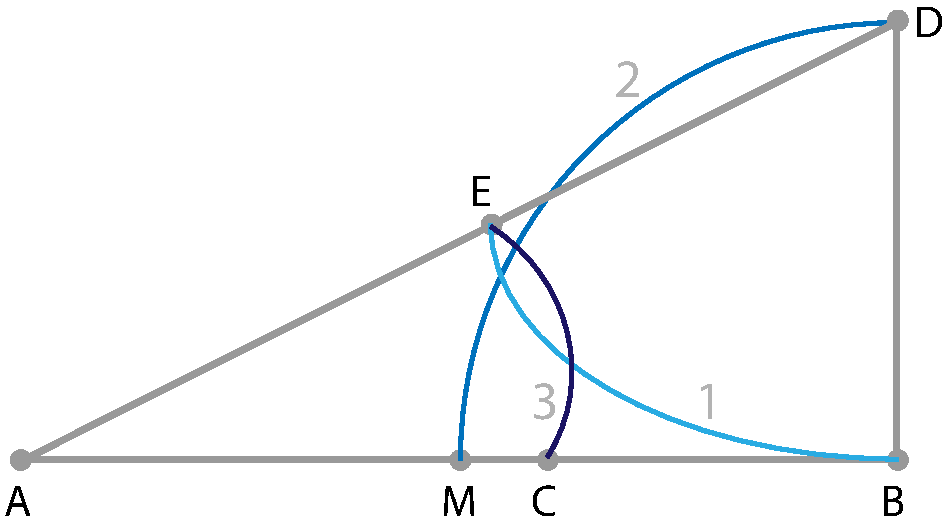
\includegraphics[width=7.5cm]{figuras/10-24.pdf}
	\vspace{-1em}
\end{figure}
\obligatorio\dem{La construcción está contenida en la figura. Se puede demostrar la igualdad por el \tma{de Pitágoras}, escribiendo todo en función de $AB$:
$$AB^2 + \left(\frac{1}{2}AB\right)^2 = AD^2 = (AC + \frac{1}{2}AB)^2$$
$$AB^2 + \cancel{\frac{1}{4}AB^2} = AC^2 + \cancel{\frac{1}{4}AB^2} + ACAB = AC^2 + (AB-BC)AB$$
$$\cancel{AB^2}=AC^2+\cancel{AB^2}-ABBC\iff AC^2 = AB\cdot BC$$
}

\tma{10.27, 10.28} Sea $\triangle ABC$ un triángulo isósceles tal que $AB = AC$ y $\measuredangle B = \measuredangle C = 2\measuredangle A$. Entonces $\frac{AB}{BC}$ es la razón áurea. Además, este triángulo puede construirse con regla y compás.

\obs{10.29}/\cor{10.30} El ángulo $\measuredangle A$ del triángulo áureo es $\pi/5$. Por tanto, se puede construir un pentágono regular con lados congruentes a $[A,B]$.

\tma{10.31} Un polígono regular de $n$ lados se puede construir con regla y compás sii la factorización de $n$ en números primos tiene la forma $n = 2^kp_1p_2\cdots p_m$, con $p_i$ de la forma $2^{2^s}+1$, y son primos distintos. Así, los lados polígonos construibles son $3,4,5,6,8,10,12,15,16,17, \cdots$.



 

\end{multicols*}\pagebreak
	
	\begin{multicols*}{2}
	[\section{Geometría euclidiana espacial}]
	\defi{11.0} $\E$ es el conjunto de puntos en un espacio tridimensional. La distancia $d$ es la aplicación $\E \times \E \rightarrow \R_+$.

\axioma{E1} $(\E,d)$ es un espacio métrico.

\defi{11.1} Una recta $r$ y su segmento $[A,B] = \{X \in \E \;|\; d(A,X) + d(X,B) = d(A,B) \}$ son similares que en $\P$. Una recta cumple:
\begin{itemizex}
	\item contiene al menos dos puntos distintos.
	\item Para toda terna $A,B,C$ en $r$, $A,B,C$ están alineados.
	\item Si $A,B \in r$ distintos, y $X \in \E$, si $X\in r$, $A,B,X$ están alineados.
\end{itemizex} 

\defi{11.2} Un \textbf{plano} $\pi \in \E$ es un subconjunto que, con la distancia $d$ restringida a $\pi$, cumple los axiomas de la geometría euclidiana plana.

\axioma{E2 [de los planos]}   
\begin{itemizex}
	\item Al menos existe un plano en $\E$.
	\item Para todo plano $\alpha$ existe un punto $P \in \E-\alpha$.
	\item Para $X,Y,Z \in \E$ distintos existe un plano $\alpha \in \E$ que los contiene. Si no están alineados, $\alpha$ es único, y se denota por $\alpha_{XYZ}$.
	\item Si $\alpha, \beta \in \E$ son planos distintos, cortan en una recta.
\end{itemizex}

\tma{11.4} Si $\alpha$ es un plano y $A,B \in \alpha$, entonces $r_{AB} \in \alpha$.

\obs{11.5} Por dos rectas que cortan, o por una recta y un punto que no pasa por ella, pasa exactamente un plano.

\defi{11.6}/\obs{11.7} Dos rectas $r,s$ son \textbf{paralelas} si coinciden o están contenidas en un plano y son paralelas en él. Dos rectas disjuntas pueden no ser paralelas, si no están en el mismo plano.

\defi{11.8} Una recta $l$ es \textbf{ortogonal} a un plano $\alpha$ en un punto $P$ ($l\perp_P\alpha$) si $l$ es ortogonal a toda recta de $\alpha$ que pase por $P$.
 
 \tma{11.10} Sea $r$  y $P \in r$, entonces existe un plano único $\pi$ que pasa por $P$ y es perpendicular a $r$.
 
 \tma{11.12} Sea $\alpha$ un plano y $P \in \alpha$. Existe una única recta ortogonal a $\alpha$ que pase por $P$.
 
 \tma{11.13} Sean $r,s$, y $r$ es ortogonal a $\alpha$. Si $s$ es paralela a $r$, entonces es ortogonal a $\alpha$.
 
\tma{11.15} Sea $\alpha$ y $P \in \E$. Existe una única recta $r$ tal que $P \in r$ y $r\perp \alpha$.  
 
 \defi{11.16}  Dos planos $\alpha, \beta$ son ortogonales, $\alpha \perp \beta$ si existe al menos una recta $a \in \alpha$ verificando $a \perp \beta$.
 
 \tma{11.17} Para los planos $\alpha, \beta \in \E$ se tiene
 \begin{itemizex}
 	\item $\alpha \perp \beta \iff \beta \perp \alpha$
 	\item $\alpha \perp \beta$ sii para todo $P  \in \alpha$ la única recta $a \perp \beta$ pasando por $P$ es´ta en $\alpha$.
 \end{itemizex}

\tma{11.18} Sea $\lambda$ un plano y $c$ una recta en $\E$. Existe un plano $\gamma \perp \lambda$ pasando por $c$. Si $c$ no es ortogonal a $\lambda$, $\gamma$ es único.

\defi{11.19} Dados dos planos $\pi_1, \pi_2$ en $\E$, $\pi_1$ y $\pi_2$ son \textbf{paralelos}
 si $\pi_1 = \pi_2$ o $\pi_1 \cap \pi_2 =  \emptyset$.
 
 \tma{11.20} Si $\pi_1 \parallel \pi_2$ toda recta ortogonal a $\pi_1$ lo es a $\pi_2$.'
 
 \ej{11.2} Sean $a,b,c$ tres rectas en $\E$. Si $a\parallel b$ y $b\parallel c$ entonces $a\parallel c$.
 
 \ej{11.3} Si $a,b$ son dos rectas no paralelas en $\E$, entonces existe una única recta $l$ ortogonal a $a$ y $b$.
 
 \ej{11.4/11.5} Si $\pi_1$ y $\pi_2$ son paralelos y $\alpha$ es ortogonal a $\pi_1$, entonces $\alpha$ es ortogonal a $\pi_2$. Si $\beta$ no es paralelo a $\pi_1$, entonces $\beta$ tampoco es paralelo a $\pi_2$\end{multicols*}\pagebreak
	
	\pagebreak
	\textcolor{gris}{\textit{Page intentionally left in blank}}
	\newpage
	\pagebreak
	
	\begin{multicols*}{2}
	[\section{Isometrías en el espacio}]
	\defi{12.0} La igual que en $\P$, una \textbf{isometría} es una aplicación $g:\E \rightarrow\E$ biyectiva que conserva las distancias.

\tma{12.1} Sea $g$ una isometría y $A, B \in \E$. Entonces $g([A,B]) = [g(A), g(B)]$ y $g(r_{AB}) = r_{g(A)g(B)}$.

\tma{12.2} Sea $g$  y $\pi \in \E$, entonces $g(\pi) \in \E$.

\tma{12.3} Si $A,B,C \in \E$ no son alineados, entonces $g(\pi_{ABC}) = \pi_{g(A)g(B)g(C)}$

\tma{12.4} Sea $l$ una recta y $\alpha, \beta$ planos en $\E$.
\begin{itemizex}
	\item $l\perp \alpha \iff g(l) \perp g(\alpha)$
	\item $\beta \perp \alpha \iff g(\beta) \perp g(\alpha)$
\end{itemizex}

\defi{12.5 [Reflexión sobre plano]} Sea $\alpha \in \E$. Dado $P \in \E$ sea $t_P$ ortogonal a $\alpha$ que pasa por $P$, y $\pi_{\alpha}(P) = t_P \cap \alpha$. La \textbf{reflexión con base $\alpha$} de $P$, o $\sigma_\alpha(P)$, es el punto tal que $\pi_\alpha(P) = \m[P, \sigma_\alpha(P)]$   

\obs{12.6}/\tma{12.7} $\sigma_\alpha$ es una biyección, y $\sigma_\alpha \circ \sigma_\alpha (P) = P$. Además, $\sigma_\alpha(P) = P \iff P \in \alpha$. $\sigma_\alpha$ es una isometría.

\tma{12.8} Sea $\pi$ un plano y $\sigma_r$ una reflexión en $\pi$ respecto a $r$. Existe una reflexión $\sigma_\alpha \in \E$ de modo que $\sigma_\alpha$ restringida a $\pi$ coincide con $\sigma_r$.

\cor{12.9} Sea $g$ una isometría de un plano $\pi$. Entonces existe una isometría $\tilde{g}(X) = g(X)$ para todo $X\in\pi$.

\cor{12.10} Sean $\pi_1$ y $\pi_2$ dos planos del espacio. Existe una isometría $g$ tal que $g(\pi_1) = \pi_2$, y se puede tomar $g$ como reflexión.

\lema{12.11} Sea $g\in \iso{(\E)}$. Si $A\neq B$ son fijos en $g$, entonces $r_{AB}$ es fija en $g$.

\tma{12.12} Sea $g$, y sea $\alpha$ el plano pasando por $A,B,C$. Si $A,B,C$ son fijos en $g$, entonces $g = \sigma_\alpha$ o $g = \text{id}_{\E}$.

\cor{12.13} Sean $A^1,A^2, A^3, A^4 \in \E$, no situados en el mismo plano; y sean $g,h\in \iso{(\E)}.$ Si $g(A^i) = h(A^i)$ para todo $i$, entonces $g = h$.

\tma{12.15} 
\begin{itemizex}
	\item Sea $\rho \in \iso{(\E)}$ una rotación de eje $r$. Para todo plano $\alpha$ conteniendo a $r$, existen planos $\beta, \beta'$ conteniendo a $r$, únicos, tales que $\rho(\alpha) = \sigma_\beta\sigma_\alpha = \sigma_\alpha\sigma_{\beta'}$.
	\item Sea $\tau$ una traslación paralela a una recta $c$. Para todo plano $\alpha \perp c$ existen planos $\beta, \beta'$, únicos, tales que $\tau =\sigma_\beta\sigma_\alpha = \sigma_\alpha\sigma_{\beta'}$.
\end{itemizex}

\ej{12.1} Si $g,h\in\iso{(\E)}$ son rotaciones con ejes ortogonales al mismo plano $\lambda$, entonces $gh$ o bien es una rotación con eje ortogonal a $\lambda$, o una traslación paralela a rectas contenidas en $\lambda$ o la identidad.

\ej{12.2} Las rotaciones forman una clase de congruencia, con el \textbf{ángulo de rotación $\rho$.} Si $\angle V$ es el ángulo formado por la semirrectas de $\alpha \cup \lambda$ y $\beta \cup\lambda$ (siendo $\alpha, \beta$ los planos de reflexión, y $\lambda$ ortogonal a $\alpha, \beta$), entonces $2\angle V$ es el ángulo de rotación. Si el ángulo de rotación es llano, entonces $\rho$ es una \textbf{media vuelta}.

\ejem{12.18} Tomando un plano $\pi$ y componiendo la reflexión $\sigma_\pi$ con una rotación $\rho$ de eje $a \perp \pi$, se obtiene la isometría $\phi = \sigma_\pi \rho = \rho\sigma_\pi$


\ejem{12.20} Una \textbf{reflexión central} es una isometría entre un plano $\alpha$ y una recta $r\perp \alpha$, en un punto $P = r \cap \alpha$:  $\sigma_P= \sigma_\alpha \rho_r$. 
La reflexión central cumple 
\begin{itemizex}
	\item Para todo $X \in\E$, $\m[X, \sigma_P(X)] = P$.
	\item $\sigma_P \circ \sigma_P= \text{id}_\E$.
	\item Para cualquier $\beta, s$ tal que $\beta\perp_P s$, $\sigma_\beta\rho_s = \rho_s\sigma_\beta$.
\end{itemizex}

\ej{12.4} \begin{itemizex}
	\item El producto de dos reflexiones centrales $\sigma_P, \sigma_Q \; (P\neq Q)$ es una traslación paralela a la recta $r_{PQ}$.
	\item Sea $\tau$ una traslación. Para todo $S \in \E$ existen puntos $B, B' \in \E$ únicamente determinados tales que $\tau = \sigma_A\sigma_{B'} = \sigma_B\sigma_A$.
\end{itemizex}


\ejem{12.21} Un \textbf{movimiento helicoidal} es una composición de una rotación con eje $r$ y una traslación paralela a dicho eje: $h = \tau \circ \rho = \rho \circ \tau$.
 
\ejem{12.22} Una \textbf{reflexión con deslizamiento} es una composición de una reflexión $\sigma_\alpha$ y una traslación $\tau$ paralela a la recta $r \subset \alpha$: $d = \tau\sigma_\alpha = \sigma_\alpha\tau$.


\tma{12.19} Las únicas isometrías en $\iso{(\E)}- \text{id}_\E$ con puntos fijos son las refleiones, rotaciones, o reflexiones-rotaciones.

\tma{12.23} Las isometrías de $\E$ sin puntos fijos son las traslaciones, movimientos helicoidales y reflexiones con deslizamiento.

\ej{12.5} Resumen de isometrías:

\begin{tabular}{ccccc}
	Puntos fijos & $\emptyset$ & $A$ & $a$ & $\alpha$\\ \midrule
	par  & $\tau$ /  $h$ & & $\rho$ & \\
	impar & $d$ & $\phi$ & & $\sigma$ \\
\end{tabular}
\end{multicols*}\pagebreak
	
	\begin{multicols*}{2}
	[\section{Poliedros}]
	\defi{13.1} Un \textbf{poliedro} $\PP$ es un conjunto finito de polígonos $\{C_kw\}$. Los polígonos de $\PP$ se llaman caras, los lados del polígono se llaman aristas o lados, y los vértices tienen el mismo nombre. Todo poliedro cumple:
\begin{itemizex}
	\item Dos caras de un poliedro o bien no se cortan, y tienen un único vértice en común, o un lado en común.
	\item Cada arista es un lado de dos polígonos de $\PP$.
	\item Las caras que comparten un vértice en común $V$ se pueden ordenar en una sucesión $C_1, \cdots, C_r$ de modo que $C_i$ y $C_{i+1}$ son adyacentes. 
	\item Dadas dos caras $C_i, C_j$ existe una sucesión finita de caras $C_1, \cdots, C_r$ tal que $C_i = C_1, C_r = C_j$.
\end{itemizex}

\defi{13.2} Un poliedro es \textbf{convexo} si toda recta no contenida en ninguno de los planos que contienen a las caras corta a lo más en dos puntos a las caras.

\defi{13.3} Un \textbf{ciclo poligonal} $\C$ es un conjunto finito de segmentos (lados) con un conjunto finito de puntos (vértices) que verifican
\begin{itemizex}
	\item Dos segmentos o no se cortan o tienen un extremo en común.
	\item Los lados de $\C$ se pueden escribir como una sucesión finita de la forma $[V_1,V_2], [V_2,V_3],\cdots, [V_{r-1},V_r],[V_r,V_1]$.
\end{itemizex}

\defi{13.4} Sea $\L$ un conjunto formado por algunos lados de $\PP$. Dadas dos caras $P$ y $P'$ de $\PP$ decimos que están \textbf{conectadas} en $\PP - \L$ si existe una sucesión de polígonos de $\PP$, $P = P_1, \cdots, P_r = P'$ de modo que $P_i$ y $P_{i+1}$ tienen un lado en común que no está en $\L$. Si $C$ es una cara de $\PP$, la componente conexa de $\PP - \L$ que contiene a $C$ es el subconjunto de $\PP$ formado por los polígonos de $\PP$ que están conectados con $C$ en $\PP-\L$.

\tma{13.5} Sea $\PP$ un poliedro convexo y $\C$ un ciclo de $\PP$, entones hay exactamente dos componentes convexas en $\PP-\C$.

\tma{13.9 [Descartes-Euler]} Sea $\P$ un poliedro convexo, con $c$ caras, $l$ lados y $v$ vértices, entonces:
$c-l+v = 2$

\defi{13.11} Un \textbf{poliedro regular} es un poliedro convexo contodas las caras congruentes a un mismo polígono regular y cada vértice está en un mismo número de caras. Decimos que un poliedro regular tiene tipo $\{n, m\}$ si sus caras son polígonos regulares con $n$ lados y cada vértice es vértice exactamente de $m$ caras.

\begin{tabular}{ccccc}
	Nombre & Tipo & $c$ & $l$ & $v$ \\\midrule
	Tetraedro & $\{3,3\} $& 4 & 6 & 4 \\
	Octaedro & $\{3,4\}$ & 8 & 12 & 6 \\
	Cubo & $\{4,3\}$ & 6 & 12 & 8 \\
	Dodecaedro & $\{3,5\}$ & 20 & 30 & 12 \\
	Icosaedro & $\{5,3\}$ & 12 & 30 & 20 \\
\end{tabular}

\tma{13.14} Dado un real $l>0$ existe un poliedro regular de tipo $\{3,3\},\{3,4\},\{4,3\},\{3,5\},\{5,3\}$, cuya arista mide $l$. Además, si $\PP_1$ y $\PP_2$ son dos poliedros del mismo tipo y con la misma longitud de arista entonces existe una isometría $\eta$ tal que $\eta(\PP_1) = \PP_2$.

\tma{13.16} Sea $V, W$ dos vértices de un poliedro regular $\PP, a, b$ dos aristas, de modo que $a$ tiene por uno de sus extremos $V$ y $b$ tiene por extremo $W$, por último sea $C_1$ una cara que tiene a $a$ como uno de sus lados y $C_2$ una cara que tiene a $b$ como lado. Existe una simetría $\theta$ de $\PP$ tal que
\[\theta(V) = W \;\; \theta(a)=b \;\; \theta(C_1) = C_2  \]

\defi{} Dado un polígono $\PP$ regular, el polígono \textbf{dual} de $\PP$, o $\PP*$, es aquel formado por la unión de los centros de las caras que forman los triedos (tres polígonos que comparten el mismo vértice $V$).

\defi{} Si consideramos el plano $\pi$ ortogonal a $r_{VW}$, siendo $V,W$ los dos vértices de un lado en común entre dos caras$P_1, P_2$ de $\PP$. $\pi$ pasa, por ejemplo, por $\m[V,W]$. Llamamos \textbf{ángulo diédrico} al ángulo de $\pi$ con vértice en $\m[V,W]$ y cuyos lados contienen a los segmentos que son las intersecciones de $P_1$ y $P_2$ con $\pi$.

\subsection{Simetrías de poliedros}
Existen tres tipos de simetrías

\textbf{Rotaciones}
\begin{itemizex}
	\item Rotaciones con eje ortogonal a una cara $C$ de $\PP$ y pasa por el el centro de $C$; con ángulos de rotación $2\pi r/n\;,r = 1, \cdots, n-1$.
	\item Rotaciones cuyo eje pasa por un vértice $V$ de $\PP$ y es ortogonal al polígono formado por los centros de las caras de $\PP$ que tienen a $V$ como uno de sus vértices; con ángulos de rotación $2\pi r/m\;,r = 1, \cdots, m-1$.
	\item Medias vueltas con eje $e$ que pasa por el punto medio $M$ de una arista $a$ de $\PP$. Además $e$ es ortogonal a $a$, así deja invariante la arista $a$ aunque intercambia sus extremos. $e$ es la bisectriz del ángulo formado por las dos caras $C_1, C_2$ que comparten $a$ y que pasa por $M$; permutando así $C_1$ y $C_2$.
\end{itemizex}

\textbf{Reflexiones}
\begin{itemizex}
	\item Sea $C$ una cara de $\PP$, que está contenida en un plano $\pi$.
	Cada reflexión $\sigma$ en $\pi$ se extiende a una reflexión $\eta$ en el espacio. El plano de reflexión para $\eta$ es el plano ortogonal a $\pi$ que lo corta en el eje de reflexión. Cada poliedro tiene, por cara, $n$ reflexiones si la cara es pentágono o triángulo y 2 si es cuadrado.
	\item Para el \textit{octaedro} existe una reflexión sobre el cuadrado interno que forman las dos pirámides.
\end{itemizex}

\textbf{Reflexiones-rotaciones}
\begin{itemizex}
	\item Tipo A: tanto la reflexión como la rotación son simetrías. 
		\subitem Cubo y octaedro: rotación con ángulo $\pi/2$ o $\pi$ y con ejes que pasa por el centro de las caras opuestas (cubo) o por los puntos opuestos de las pirámides, o del cuadrado interno (octaedro).
		\subitem Dodecaedro e icosaedro: rotación con ángulos $\pi/3, \pi/5, 3\pi/5$ y con eje que pasa por los puntos medios de dos caras opuestas o dos vértices opuestos.
	\item Tipo B: ni la reflexión ni la rotación son simetrías, pero la combinación de ambas sí.
		\subitem Tetraedro: rotación con ángulo $\pi/2$ y con eje que pasa por los puntos medios de las aristas.
		\subitem Cubo: rotación con ángulo $\pi/3$ y con eje que pasa por los puntos opuestos del poliedro.
		\subitem Octaedro: rotación con ángulo $\pi/3$ y con eje que pasa por los puntos medios de dos caras opuestas.
		\subitem Dodecaedro e icosaedro: rotación con ángulo $\pi$ y con eje que pasa por los puntos medios de dos caras opuestas o dos vértices opuestos.
\end{itemizex}\end{multicols*}\pagebreak	

	\begin{multicols*}{2}
	[\section{Geometría analítica}]
	\defi{14.1} Un paralelogramo $\square PABC$ se llama \textbf{rectángulo} si $r_{PA} \perp r_{PC}$


\obs{14.3} Un sistema de \textbf{coordenadas cartesianas} es un par de rectas $l^1$, $l^2 \subset \P$ cortándose ortogonalmente en un punto $O$, llamado \textbf{origen}, siendo así $l^1,l^2$ los \textbf{ejes} [El sistema es construible porque el \tma{2.29} garantiza la existencia de $l_2 \perp l_1$ único pasando por $O$].
Por el \axioma{P3} existen aplicaciones
$$\gamma_k: l^k \rightarrow \R, \;\; k = 1,2$$
tales que 
$$X,Y \in l^k \rightarrow d(X,Y) = \abs{\gamma_k(X) - \gamma_k(Y)}$$
Además, podemos elegir puntos $E^k$ tales que $\gamma_k(O) = 0\;\text{y}\; \gamma_k(E^k)=1$.
Este sistema de coordenadas $OE^1E^2$ es orientado, y a todo punto $A \in \P$ se le pueden asociar dos reales $a_1, a_2$ tales que cada $a^k$ es ortogonal a $l^k$, de modo que $a_k = \gamma_k(A^k)$; y se puede determinar la aplicación de coordenadas $\Gamma(A) = (a_1,a_2)$.



\obs{[Coordenadas en $\E$]} Un sistema de coordenadas en el espacio $\E$ es una terna de rectas $l^1,l^2,l^3$ ortogonales entre sí, los ejes, con un origen $O$; los puntos $E^k$ tales que $d(O, E^k) = 1$ que generan el sistema de coordenadas $OE^1E^2E^3$, y las aplicaciones $\gamma_k$ y $\Gamma$ similares a las de la $\obs{14.3}$ pero con una dimensión más. 

\tma{14.4/14.6/14.7} La aplicación $\Gamma:\P\rightarrow \R^2$ es biyectiva. Si $A,B$ son dos puntos, y $\Gamma(A) = (a_1,a_2)\;;\;\Gamma(B) = (b_1,b_2)$, entonces 
$$d(A,B)^2 = (a_1-b_1)^2+(a_2-b_2)^2$$
Para $\E$, $\Gamma:\E\rightarrow \R^3$ también es biyectiva, y la distancia entre $A, B$ viene dada por 
$$d(A,B)^2 = (a_1-b_1)^2+(a_2-b_2)^2+(a_3-b_3)^2$$

\cor{14.5}/\obs{14.8} El espacio métrico $(\P,d)$ es isométrico a $(\R^2,d_E)$ y $\Gamma:\P\rightarrow\R^2$ es una isometría. El espacio métrico $(\E,d)$ es isométrico a $(\R^3,d_E)$ y $\Gamma:\E\rightarrow\R^3$ es una isometría.

\defi{[Espacio Euclidiano $\R^n$]} El espacio $\R^n$ es el conjunto $\R^n = \{X=(x_1, \cdots, x_n) \; | \; x_i \in \R;\; i = 1,\cdots, n \}$. El conjunto tiene una estructura de \textbf{espacio vectorial} con las operaciones
\[X+Y \equiv (x_1+y_1,\cdots, x_n+y_n) \;;\; X,Y \in \R^n \]
\[\lambda X = (\lambda x_1, \cdots, \lambda x_n) \;;\; \lambda \in \R \]

\defi{14.9 [Distancia euclidiana en $\R^n$]} Para dos puntos $X,Y \in \R^n$ la métrica euclidiana es la aplicación  $d: \R^n \times \R^n \rightarrow \R^+$ tal que
$$d(X,Y) \equiv \left(\sum_{i = 1}^{n}(x_i-y_i)^2\right) ^{1/2}$$

\defi{14.10} El \textbf{producto escalar} de $X,Y$ es
$$\prodvec{X,Y} = X\cdot Y \equiv \sum_{i = 1}^nx_iy_i$$
La \textbf{norma} es la operación 
$$||X||\equiv \langle X,X \rangle^{1/2} = \sum_{i = 1}^nx_i^2$$

\tma{14.11} Para $X,X',Y,Y' \in \R^n$ y $\lambda \in \R$:
\begin{itemizex}
	\item $\prodvec{X,X} \ge 0 \; ;\; \prodvec{X,X} = 0 \iff X = 0$
	\item $\prodvec{X,Y} = \prodvec{Y,X}$
	\item $\prodvec{\lambda X, Y} = \lambda \prodvec{X,Y} = \prodvec{X, \lambda Y}$
	\item $\prodvec{X+X' , Y} = \prodvec{X,Y}+\prodvec{X',Y}\;;\;
	\prodvec{X , Y+Y'} = \prodvec{X,Y}+\prodvec{X,Y'}$
\end{itemizex}

\obs{14.12} El producto escalar y la distancia están relacionados:
\begin{itemizex}
	\item $d(X,Y) = ||X-Y|| = \sqrt{\prodvec{X-Y,X-Y}}$
	\item $d(X,-Y) = ||X+Y||$
	\item $\prodvec{ X, Y} = \frac{1}{4}(||X+Y||^2 - ||X-Y||^2)$
	\item $\prodvec{X, Y} = \frac{1}{2}(||X||^2 + ||Y||^2 - ||X-Y||^2)$
\end{itemizex}

\tma{14.13}  Sea $V \in \R^n\;, \;V \neq 0$. Para todo $U \in \R^n$ existe un único $\lambda_U \in \R$ y un único $V_{U}^\perp$ tales que
$$U = \lambda_UV + V_{U}^\perp\;;\; \prodvec{V, V_{U}^\perp} = 0$$
Además, $\lambda_U$ y $V_U^\perp$ se expresan como
$$\lambda_U= \frac{\prodvec{U,V}}{||V||^2} = \frac{\prodvec{U,V}}{\prodvec{V,V}}\;;\; V_U^\perp = U - \lambda_UV$$
\dem{Por la definición de $U$ tenemos que $\prodvec{U,V} = \prodvec{\lambda_UV+V_U^\perp,V} = \lambda_U\prodvec{V,V}+\cancel{\prodvec{V_U^\perp,V}}\iff\lambda_U= \frac{\prodvec{U,V}}{||V||^2}$\linebreak
	Por otra parte, $\prodvec{V_U^\perp, V} = \prodvec{U-\lambda_UV,V} = \prodvec{U,V} - \lambda_U\prodvec{V,V}= \prodvec{U,V} - \prodvec{U,V}\frac{||V||^2}{||V||^2} = 0$}
\begin{figure}[H]
	\centering
	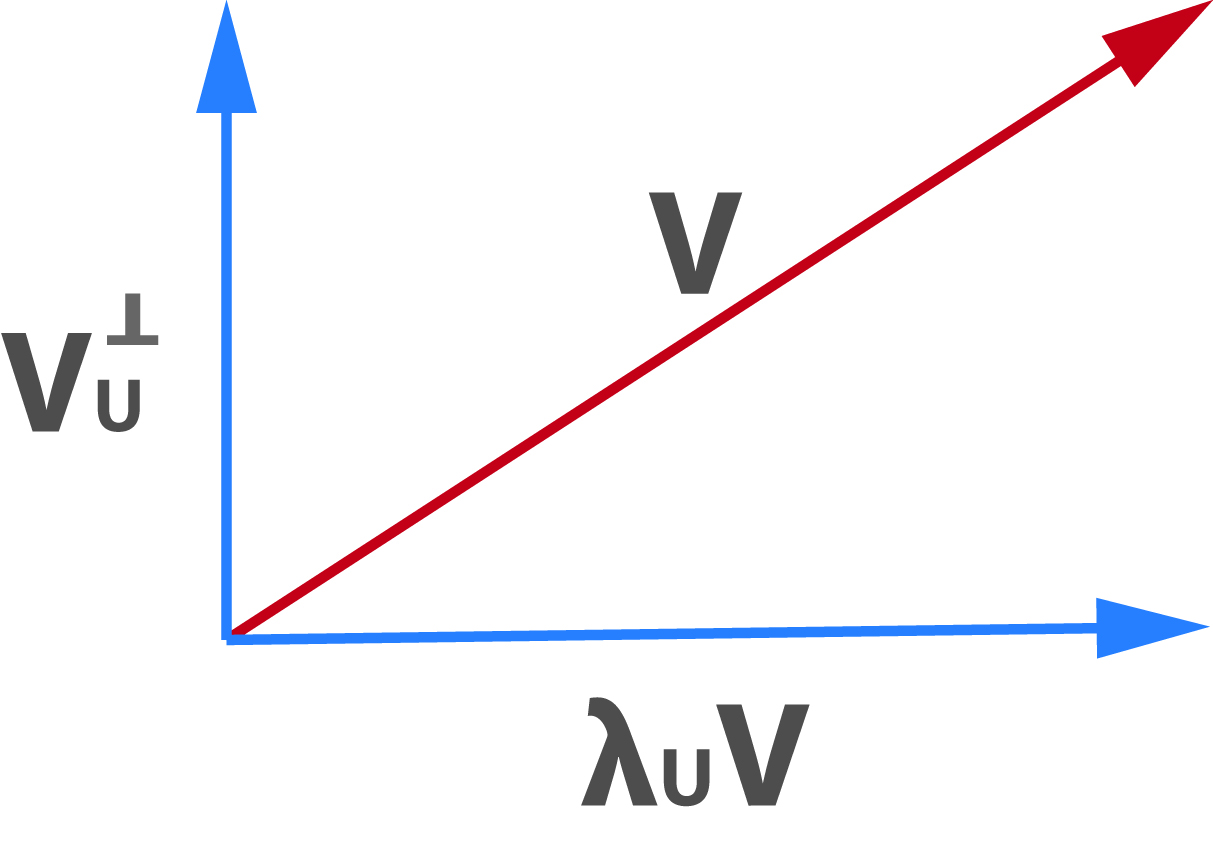
\includegraphics[width=5.5cm]{figuras/13-13.jpg}
	\vspace{-1em}
\end{figure}
\tma{14.14} $(\R^n,d)$ es un espacio métrico: para cada terna $X,Y,Z\in\R^n$ se satisface
\begin{itemizex}
	\item $d(X,Y) \ge 0\;;\; d(X,Y) = 0 \iff X=Y$
	\item $d(X,Y) = d(Y,X)$
	\item $d(X,Z) + d(Z,Y) \ge d(X,Y)$
\end{itemizex}
\dem{Para la tercera afirmación: $V = Y-X$. Segun 14.13, existen $\lambda, W$ tales que $Z-X = \lambda V+W\;;\;\prodvec{V,W} = 0$. Si $Z-Y = Z-X-(Y-X) = (\lambda-1)V+W$ y manipulamos las distancias:
$$||Z-X||^2 = \prodvec{\lambda V+W,\lambda V+W} = \lambda^2||V||^2 + ||W||^2$$
$$||Z-Y||^2 = \prodvec{(\lambda-1)V + W, (\lambda - 1)V + W} = (\lambda - 1)^2||V||^2 + ||W||^2 $$
Y, por tanto
$$||Z-X||+||Z-Y|| \ge |\lambda|\cdot||V|| + |\lambda-1|\cdot||V|| \ge ||V|| = ||Y-X||$$}
\obs{14.15} Para $A,B \in \R^n$ se llama \textbf{segmento de recta}, $[A,B]$ al conjunto
$$[A,B] = \{X \in \R^n \;|\; d(A,X) + d(X,B) = d(A,B) \}$$
o, empleando el \tma{14.14}
$$[A,B] = \{Z \in \R^n\;|\; Z = A + \lambda(B-A)\;,\; \lambda\in [0,1]\}$$

\ej{14.2 [Desigualdad de Cauchy-Schwarz]} Sean $U,V \in \R^n,\; V\neq 0$. Entonces
$$\prodvec{U,V}^2 \le ||U||^2\cdot||V||^2$$
y se cumple la igualdad sii $U = \lambda V$.

\end{multicols*}\pagebreak	


	 \noindent\rule{\linewidth}{0.4pt}
	 \doclicenseThis
	 
	 
	 
	 
	 
	 
	 
	 
	  	
 	
 	
 	
 	
 	
\end{document}